%% LyX 2.2.3 created this file.  For more info, see http://www.lyx.org/.
%% Do not edit unless you really know what you are doing.
\documentclass[oneside]{scrbook}
\usepackage[latin9]{inputenc}
\usepackage{fancyhdr}
\pagestyle{fancy}
\setcounter{secnumdepth}{3}
\setcounter{tocdepth}{1}
\synctex=-1
\usepackage{fancybox}
\usepackage{calc}
\usepackage{bm}
\usepackage{graphicx}
\usepackage{esint}
\usepackage[unicode=true,pdfusetitle,
 bookmarks=true,bookmarksnumbered=false,bookmarksopen=false,
 breaklinks=false,pdfborder={0 0 1},backref=section,colorlinks=false]
 {hyperref}

\begin{document}

\title{xSPDE: The Stochastic Toolbox }

\title{User's Guide v3.0}

\author{Peter D. Drummond, Rodney Polkinghorne, Simon Kiesewetter}

\maketitle

\tableofcontents{}

\chapter{Introduction\label{chap:Introduction}}

The xSPDE stochastic toolbox is an e\textbf{x}tensible \textbf{S}tochastic
\textbf{P}artial \textbf{D}ifferential \textbf{E}quation solver. It
can solve any number of simultaneous equations in any number of space
dimensions, with averaging and graphical output. This user's guide
can be used as the basis for a 3-4 hour self-taught tutorial in solving
practical stochastic problems. It includes exercises for the reader.
A full-length manual is available online. Research use of this software
is encouraged, and should be referenced to the corresponding paper\cite{Kiesewetter}.
See:\emph{ }\textbf{www.github.com/peterddrummond/xspde\_matlab.}


Stochastic equations are equations with random noise terms \cite{Gardiner,Drummond}.
They occur in in many fields of biology, chemistry, engineering, economics,
physics, meteorology and other disciplines. An ordinary stochastic
equation for a real or complex vector $\mathbf{a}$ is:

\begin{equation}
\frac{\partial\bm{a}}{\partial t}=\dot{\bm{a}}=\mathbf{A}\left(\bm{a}\right)+\underline{\mathbf{B}}\left(\bm{a}\right)\bm{w}(t).
\end{equation}
Here, $\mathbf{A}$ is a vector, $\underline{\mathbf{B}}$ a matrix,
and $\mathbf{w}$ is a real noise vector, delta-correlated in time:
\begin{eqnarray}
\left\langle w_{i}\left(t\right)w_{j}\left(t\right)\right\rangle  & = & \delta\left(t-t'\right)\delta_{ij}
\end{eqnarray}

Stochastic partial differential equations including space dependence
are also numerically soluble \cite{DrummondMortimer,KP} with xSPDE.
These are described in Chapter \ref{chap:Stochastic-partial-differential}.

xSPDE is a Matlab based software toolbox. It has functions that can
numerically solve both ordinary and partial differential stochastic
equations, and graph results of correlations and averages. There are
many equations of this type, and the xSPDE toolbox can treat a wide
range. The extensible general structure permits drop-in replacements
of the functions provided. Different simulations can be carried out
sequentially, to simulate the various stages in an experiment or other
process. It can even be used with no noise.

The code supports parallelism at both the vector instruction level
and at the thread level, using Matlab matrix instructions and the
parallel toolbox. It calculates averages of arbitrary functions of
any number of complex or real fields, as well as Fourier transforms
in time or space. It provides error estimates for both step-size and
sampling error. 

\emph{xSPDE is distributed without any guarantee, under an open-source
license. Contributions and bug reports always welcome.}

\chapter{xSPDE simulations\label{chap:Interactive-xSPDE}}

The general purpose xSPDE toolbox function co is:
\begin{itemize}
\item \textbf{xspde(in)}, the combined simulation (xSIM) and graphics (xGRAPH)
function.
\end{itemize}

\section{Running xSPDE interactively}

To simulate a stochastic equation, first make sure that either the
Matlab xSPDE toolbox is installed, or the Matlab path is pointing
to the xSPDE folder and subfolders. If not, proceed as follows:
\begin{itemize}
\item Click on the Matlab HOME tab (top left), then Set Path
\item Click on Add with Subfolders
\item Find the xSPDE folder in the drop-down menu, and select it
\item Click on close to save the path.
\end{itemize}
Next, type $clear$ to clear old data, and enter the xSPDE inputs
and functions into the command window. For the simplest of examples,
do this by cutting and pasting from an electronic file of this manual.
You can also use the Matlab built-in editor.

A typical script is as follows:

\begin{eqnarray*}
\mathtt{in.}[label1] & = & [parameter1]\\
\mathtt{in.}[label2] & = & \ldots\\
\mathtt{in.da} & = & \mathtt{@(a,w,r)}\,\,[derivative]\\
\mathtt{xspde(in)}
\end{eqnarray*}

Note the following points to remember:
\begin{itemize}
\item The notation $\mathtt{in.}[label1]=[parameter1]$ inputs a value to
the $\mathtt{in}$ data structure 
\item There are many input possibilities, and they all have default values.
\item You don't have to save the data if you just want an immediate plot 
\item The notation $\mathtt{in.da=}\mathtt{@(a,w,r)}\,\,[derivative]=..$
defines an inline function, $da/dt$. 
\item In xSPDE, $\mathtt{a}$ is the stochastic variable, $\mathtt{w}$
the random noise, and $\mathtt{r}$ the parameters. 
\item For example, $\mathtt{r.t}$ is the current time, and $\mathtt{r.x},$
$\mathtt{r.y},$ $\mathtt{r.z},$ the grid of coordinates. 
\end{itemize}

\section{Inputs}

All xSPDE simulations use a structure \emph{in} for input data. All
functions use an internally generated structure $r$, combining $in$
with other generated parameters. Any name will do for either structure,
as long as you are consistent. 

All xSPDE inputs have default values, which can be changed by typing
parameters into the \emph{in} structure. If you only need the first
value of a vector or array, just input the value that is required.

\subsection{Common xSPDE inputs}

The most common xSPDE parameters are: \\

\begin{center}
\begin{tabular}{|c|c|c|c|}
\hline 
Label  & Type  & Default value  & Description\tabularnewline
\hline 
\hline 
\emph{in.fields}  & integer vector & $1$ & Stochastic field variables\tabularnewline
\hline 
\emph{in.noises}  & integer vector & $1$ & Number of noises\tabularnewline
\hline 
\emph{in.dimension} & integer  & $1$ & Space-time dimensions\tabularnewline
\hline 
\emph{in.name}  & string  & ' '  & Simulation name\tabularnewline
\hline 
\emph{in.olabels}  & string & \emph{'a'} & Observable labels\tabularnewline
\hline 
\emph{in.da}  & function  & \emph{ 0} & The stochastic derivative\tabularnewline
\hline 
\emph{in.define}  & function  & \emph{ 0} & Defined field definition\tabularnewline
\hline 
\emph{in.initial}  & function  &  0 & Function to initialize variables\tabularnewline
\hline 
\emph{in.ensembles} & integer vector & {[}1,1,1{]} & Numbers of stochastic trajectories\tabularnewline
\hline 
\emph{in.observe}  & function & \emph{a} & Observable function(s) \tabularnewline
\hline 
\emph{in.linear}  & function & 0 & Linear interaction picture response\tabularnewline
\hline 
\emph{in.ranges} & real vector & 10  & Ranges in time and space\tabularnewline
\hline 
\emph{in.steps} & integer vector & $1$ & Time-steps per plot point\tabularnewline
\hline 
\emph{in.points}  & integer vector & 51  & Output lattice points in {[}t,x,y,z{]}\tabularnewline
\hline 
\emph{in.images}  & integer cell array & \emph{\{0,..\}}  & Movie images in time per 2D observable\tabularnewline
\hline 
\emph{in.transforms}  & vector cells  & \emph{ \{{[}0 0 0 0{]},..\}}  & Fourier transforms in {[}t,x,y,z{]}\tabularnewline
\hline 
\end{tabular}\\
\par\end{center}

\textbf{A complete list of user inputs is given in Chapter (\ref{chap:Table-of-xSPDE}).}

\subsection{Use the dot}

Matlab formulae often require a 'dot' or a 'colon'. To multiply vectors
element-wise, like $a_{i}=b_{i}c_{i}$, the notation $a=b.*c$ indicates
all elements are multiplied. This is used in xspde to speed up calculations
in parallel. 

A formula for a stochastic field usually requires you to address the
first index - which is the field component - and treat all the other
elements in parallel. To do this, use the notation $a(1,:)$. 

Whenever a formula combines operations over spatial lattices or ensembles,
remember to \textbf{USE THE DOT}.

\section{The random walk}

The first example is the simplest possible stochastic equation: 
\begin{equation}
\dot{a}=w(t)\,,
\end{equation}

This is carried out numerically and graphed using $N=points(1)$ points.
Since the first time point stored is always the initial value, there
are $N-1$ integration steps, each of length $dt=ranges(1)/(N-1)$.
As a result, the graphs have discrete steps, and more detail is obtained
if more time steps are used. The default value is $N=51$, which is
in the $xpreferences$ file. This is adjustable by the user. It can
also be changed for a simulation, by inputting a new value of $points$. 

\subsection*{Exercises}

Remember that, unless you type \emph{clear} first, any changes to
the input structure are additive; so you will get the sum of all the
previous inputs as well as your new input.
\begin{itemize}
\item \textbf{Run the complete xSPDE script given below in Matlab. }
\end{itemize}
It is simplest to cut and paste from an electronic file into the Matlab
command window. Be careful; pasting can cause subtle changes that
may require correction. 

You should get the output in Fig (\ref{fig:The-simplest-case: Wiener}).

\begin{center}
\noindent\doublebox{\begin{minipage}[t]{1\columnwidth - 2\fboxsep - 7.5\fboxrule - 1pt}%
\texttt{in.da=@(a,w,r) w; xspde(in);}%
\end{minipage}} 
\par\end{center}

Here $in.da$ defines the derivative function, with $w$ the noise. 

\begin{figure}
\centering{}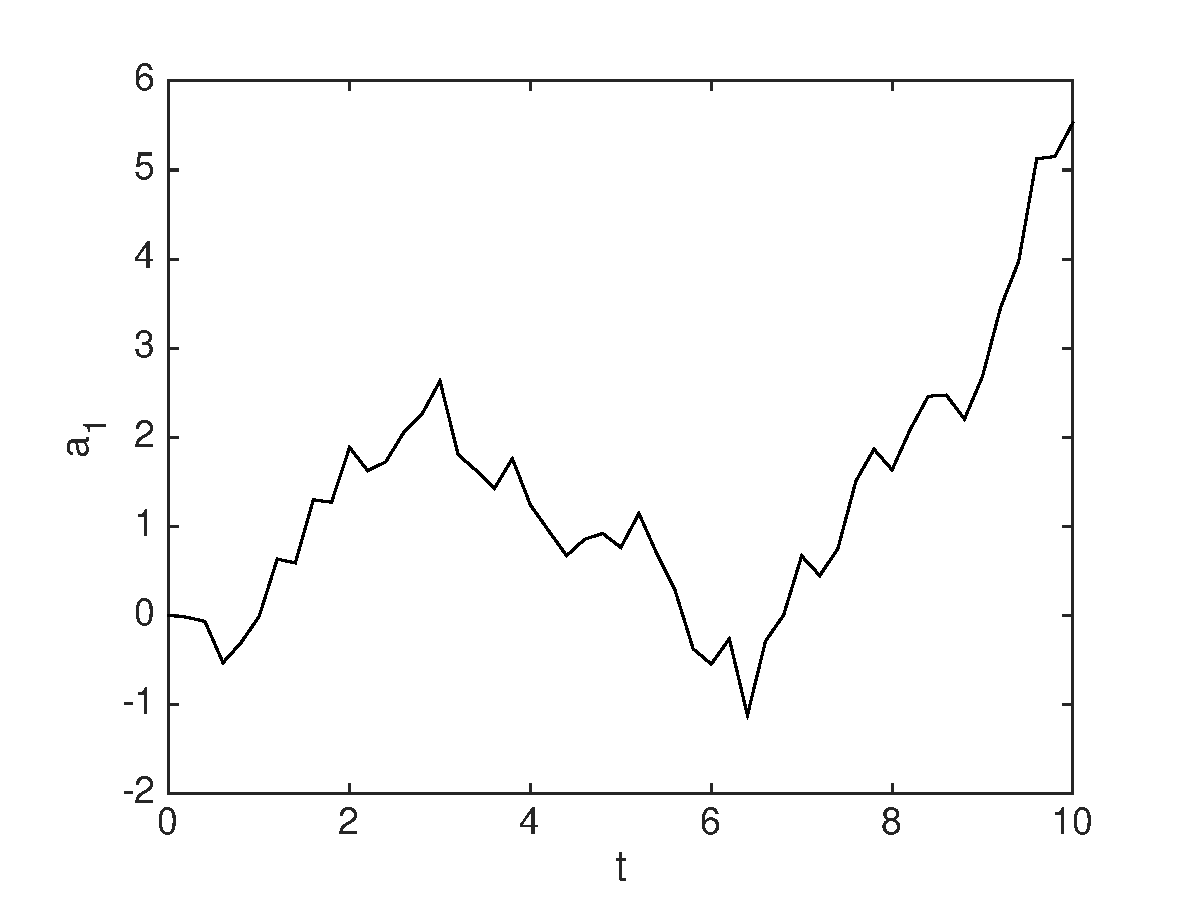
\includegraphics[width=0.75\textwidth]{Figures/Wiener_1}\caption{\label{fig:The-simplest-case: Wiener}The simplest case: a random
walk.}
\end{figure}
\begin{itemize}
\item \textbf{What do you see if you average over $10000$ trajectories
?}
\end{itemize}
\begin{center}
\noindent\doublebox{\begin{minipage}[t]{1\columnwidth - 2\fboxsep - 7.5\fboxrule - 1pt}%
\texttt{in.ensembles = 10000;}

\texttt{xspde(in);}%
\end{minipage}}
\par\end{center}
\begin{itemize}
\item \textbf{What do you see if you plot the mean square distance? Note
that variances should increase linearly with $t$.}
\end{itemize}
\begin{center}
\noindent\doublebox{\begin{minipage}[t]{1\columnwidth - 2\fboxsep - 7.5\fboxrule - 1pt}%
\texttt{in.observe = @(a,r) a.\textasciicircum{}2;}

\texttt{in.olabels = '\textless{}a\textasciicircum{}2\textgreater{}';}

\texttt{xspde(in);}%
\end{minipage}}
\par\end{center}
\begin{itemize}
\item \textbf{What if you add a force that takes the particle back to the
origin?} 
\begin{equation}
\dot{a}=-a+w(t)\,,
\end{equation}
\end{itemize}
\begin{center}
\noindent\doublebox{\begin{minipage}[t]{1\columnwidth - 2\fboxsep - 7.5\fboxrule - 1pt}%
\texttt{in.da=@(a,w,r) -a+w}

\texttt{xspde(in);}%
\end{minipage}}
\par\end{center}

\subsection*{Mathematical exercise: }
\begin{itemize}
\item If you like mathematics, then as an offline exercise, try to solve
the equivalent diffusion equation for the probability P to find the
variance $\left\langle a^{2}\right\rangle $! The equation is:
\[
\frac{\partial P\left(a\right)}{\partial t}=\left[\frac{\partial}{\partial a}+\frac{1}{2}\frac{\partial^{2}}{\partial a^{2}}\right]P\left(a\right)
\]
\end{itemize}

\section{Laser quantum noise}

Next we treat a model for the quantum noise of a single mode laser
as it turns on, near threshold:

\begin{equation}
\dot{a}=ga+bw(t)
\end{equation}
where the noise is complex, $w=\left(w_{1}+iw_{2}\right)$, so that:
\begin{equation}
\left\langle w(t)w^{*}(t')\right\rangle =2\delta\left(t-t'\right)\,.
\end{equation}

Here the coefficient $b$ describes the quantum noise of the laser,
and is inversely proportional to the equilibrium photon number. 

\subsection*{Exercises}

You should type \emph{clear }first when starting new simulations.
\begin{itemize}
\item \textbf{Solve for the case of $g=0.1$, $b=0.01$}
\end{itemize}
Most lasers have more than $100$ photons, and hence less noise! 

For this exercise, small error-bars will display on the graph. These
are calculated from the difference between using steps of size $dt$
and steps of size $dt/2$. They only appear if greater than a minimum
relative size, typically $1\%$ of the graph size, which can be set
by the user.

\begin{center}
\noindent\doublebox{\begin{minipage}[t]{1\columnwidth - 2\fboxsep - 7.5\fboxrule - 1pt}%
\texttt{clear}

\texttt{in.noises=2;}

\texttt{in.observe = @(a,r) abs(a)\textasciicircum{}2;}

\texttt{in.olabels = '\textbar{}a\textbar{}\textasciicircum{}2';}

\texttt{in.da=@(a,w,r) a+0.01{*}(w(1)+i{*}w(2));}

\texttt{xspde(in);}%
\end{minipage}}
\par\end{center}

Consider the case where the laser saturates to a steady state:

\begin{equation}
\dot{a}=\left(1-\left|a\right|^{2}\right)a+bw(t)
\end{equation}
\begin{itemize}
\item \textbf{Solve for the saturated laser case}
\end{itemize}
You should get the output graph in Fig (\ref{fig:The-laser}). 

\begin{center}
\noindent\doublebox{\begin{minipage}[t]{1\columnwidth - 2\fboxsep - 7.5\fboxrule - 1pt}%
\texttt{in.da=@(a,w,r) (1-abs(a)\textasciicircum{}2){*}a+0.01{*}(w(1)+i{*}w(2));}

\texttt{xspde(in);}%
\end{minipage}} 
\par\end{center}

\begin{figure}
\centering{}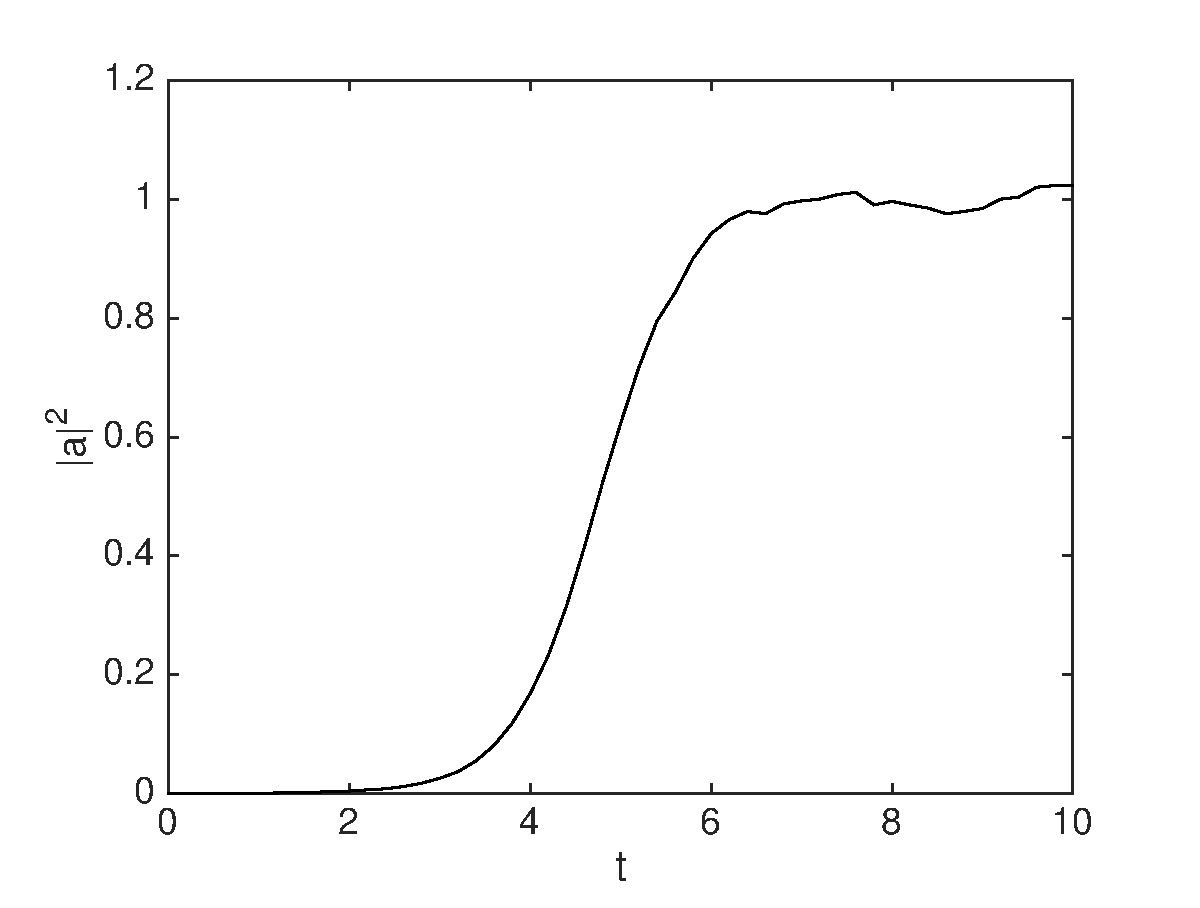
\includegraphics[width=0.75\textwidth]{Figures/Laser}\caption{\label{fig:The-laser}Simulation of the stochastic equation describing
a laser turning on.}
\end{figure}

\section{Fourier transforms and spectra}

Frequency spectra have many uses, especially for understanding the
steady-state fluctuations of any physical system. The xSPDE spectral
definition is:
\[
\tilde{a}(\omega)=\frac{1}{\sqrt{2\pi}}\int e^{-i\omega t}a(t)dt\,
\]

To get an output from a temporally Fourier transformed field, just
set $in.transforms\{n\}=1$, for the particular observable ($n$)
you need to calculate in transform space. This parameter is a cell
array. It can have a different value for every observable and for
every dimension in space-time if you have space dimensions as well.

As an example, take the random walk equation in a complex space, 
\[
\frac{da}{dt}=-a+\zeta(t)
\]
where $\zeta(t)=w_{1}(t)+iw_{2}(t)$. Use an initial condition of
$a=(v_{1}+iv_{2})/\sqrt{2}$, with $\left\langle v_{i}^{2}\right\rangle =1$,
to start near the steady state. 

For sufficiently long time-intervals, the solution in frequency space
- where $\omega=2\pi f$ is the angular frequency - is given by: 
\[
\tilde{a}\left(\omega\right)=\frac{\tilde{\zeta}(\omega)}{1+i\omega}
\]
The expectation value of the noise spectrum, in the long time-intervals
limit, is therefore: 
\begin{eqnarray*}
\left\langle \left|\tilde{a}(\omega)\right|^{2}\right\rangle  & = & \frac{1}{2\pi\left(1+\omega^{2}\right)}\int\int e^{-i\omega(t-t')}\left\langle \zeta(t)\zeta^{*}(t')\right\rangle dtdt'\,.\\
 & = & \frac{T_{eff}}{\pi\left(1+\omega^{2}\right)}
\end{eqnarray*}

The final result is obtained from the fact that the first integral
vanishes unless $t=t'$, since for small steps, $\left\langle \zeta(t)\zeta^{*}(t')\right\rangle \rightarrow2\delta\left(t-t'\right)$. 

The time integral is carried out numerically as a sum which has $N=points(1)$
time points of interval $dt$. The definition of $dt$ is therefore
$dt=T/(N-1)$, where $T=ranges(1)$. The `effective' time duration
for the Fourier transform time integrals is $T_{eff}=Ndt=T\times N/(N-1)=T+dt$.
This corresponds to a midpoint rule integration, which technically
is over the interval $[-dt/2,T+dt/2]$.

\subsection*{Exercises}
\begin{itemize}
\item \textbf{Plot the spectrum over a range of $t=100$, with $640$ points
and a random initial equation near the equilibrium value.}
\end{itemize}
The input parameters are given below. There are parallel operations
here, for ensemble averaging, so \textbf{USE THE DOT}.

\begin{center}
\noindent\doublebox{\begin{minipage}[t]{1\columnwidth - 2\fboxsep - 7.5\fboxrule - 1pt}%
\texttt{clear}

\texttt{in.points = 640;}

\texttt{in.ranges = 100;}

\texttt{in.noises = 2; }

\texttt{in.ensembles = 10000; }

\texttt{in.initial = @(v,r) (v(1,:)+1i{*}v(2,:))/sqrt(2); }

\texttt{in.da = @(a,w,r) -a + w(1,:)+1i{*}w(2,:); }

\texttt{in.observe =@(a,r) a.{*}conj(a);}

\texttt{in.transforms =1;}

\texttt{in.olabels = '\textbar{}a(\textbackslash{}omega)\textbar{}\textasciicircum{}2'; }

\texttt{xspde(in); }%
\end{minipage}} 
\par\end{center}

Note that \texttt{in.transforms =1} tells xSPDE to Fourier transform
the field over the time coordinate before averaging, to give a spectrum.
The first argument $v$ of the \emph{initial} function is a random
field, used optionally to initialize the stochastic variable. You
can transform any field in any dimension, for any number of resulting
averages. See Chapter 6 for details. 

To define as many observables as you like, use a Matlab cell array;

\begin{center}
\noindent\doublebox{\begin{minipage}[t]{1\columnwidth - 2\fboxsep - 7.5\fboxrule - 1pt}%
\texttt{in.observe\{1\} = ..;}

\texttt{in.observe\{2\} = ..;}%
\end{minipage}}
\par\end{center}
\begin{itemize}
\item \textbf{Simulate over a range of $t=200$. What changes do you see?
Why?}
\item \textbf{Change the equation to the laser noise equations. Why is the
spectrum much narrower?}
\end{itemize}

\section{Ito and Stratonovich}

The xSPDE toolbox is mainly designed to treat Stratonovich equations
\cite{Gardiner}, which are the broad-band limit of a finite band-width
random noise equation. Another type of of stochastic equation is the
Ito form, which is a limit where derivatives are evaluated at the
start of each step. If you have an Ito equation, you can either use
the Euler integration option, and set $in.step=xEuler$, or else apply
the Stratonovich correction to the drift, as outlined below. 

To emphasize the difference, an Ito equation is often written as a
difference equation:

\begin{equation}
d\mathbf{a}=\mathbf{A}^{I}\left[\mathbf{a}\right]+\underline{\mathbf{B}}\left[\mathbf{a}\right]\cdot d\bm{w}(t).
\end{equation}
Here $\left\langle dw_{i}\left(\bm{x}\right)dw_{j}\left(\bm{x}'\right)\right\rangle =\delta_{ij}dt$. 

When $\bm{\mathsf{B}}$ is constant, the two methods are identical.
If $\bm{\mathsf{B}}$ is not constant, the Ito drift term $\mathbf{A}^{I}$
is different to the corresponding Stratonovich one. The relationship
is: 
\begin{eqnarray}
A_{i} & = & A_{i}^{I}-\frac{1}{2}\sum_{j,m}\frac{\partial B_{ij}}{\partial a_{m}}B_{mj}\,.
\end{eqnarray}

\section{Financial calculus}

A well-known Ito stochastic equation is the Black-Scholes equation,
used to price financial options. It describes the fluctuations in
a stock value: 
\begin{equation}
da=\mu a\,dt+a\sigma\,dw,
\end{equation}
where $\left\langle dw^{2}\right\rangle =dt$. Since the noise is
multiplicative, the equation is different in Ito and Stratonovich
forms of stochastic calculus. 

The corresponding Stratonovich equation, as used in xSPDE for the
standard default integration routine is: 
\begin{equation}
\dot{a}=\left(\mu-\sigma^{2}/2\right)a+a\sigma w(t).
\end{equation}

\subsection*{Exercises}
\begin{itemize}
\item \textbf{Solve for a startup with a volatile stock having $\mu=0.1,\,\sigma=1$.}
\end{itemize}
An interactive xSPDE script in Matlab is given below with an output
graph in Fig (\ref{fig:The-Black-Scholes}), Note the spiky behaviour,
typical of multiplicative noise, and also of the risky stocks in the
small capitalization portions of the stock market.

\begin{center}
\noindent\doublebox{\begin{minipage}[t]{1\columnwidth - 2\fboxsep - 7.5\fboxrule - 1pt}%
\texttt{clear}

\texttt{in.initial=@(v,r) 1}

\texttt{in.da=@(a,w,r) -0.4{*}a+a{*}w}

\texttt{xspde(in)}%
\end{minipage}} 
\par\end{center}

\begin{figure}
\centering{}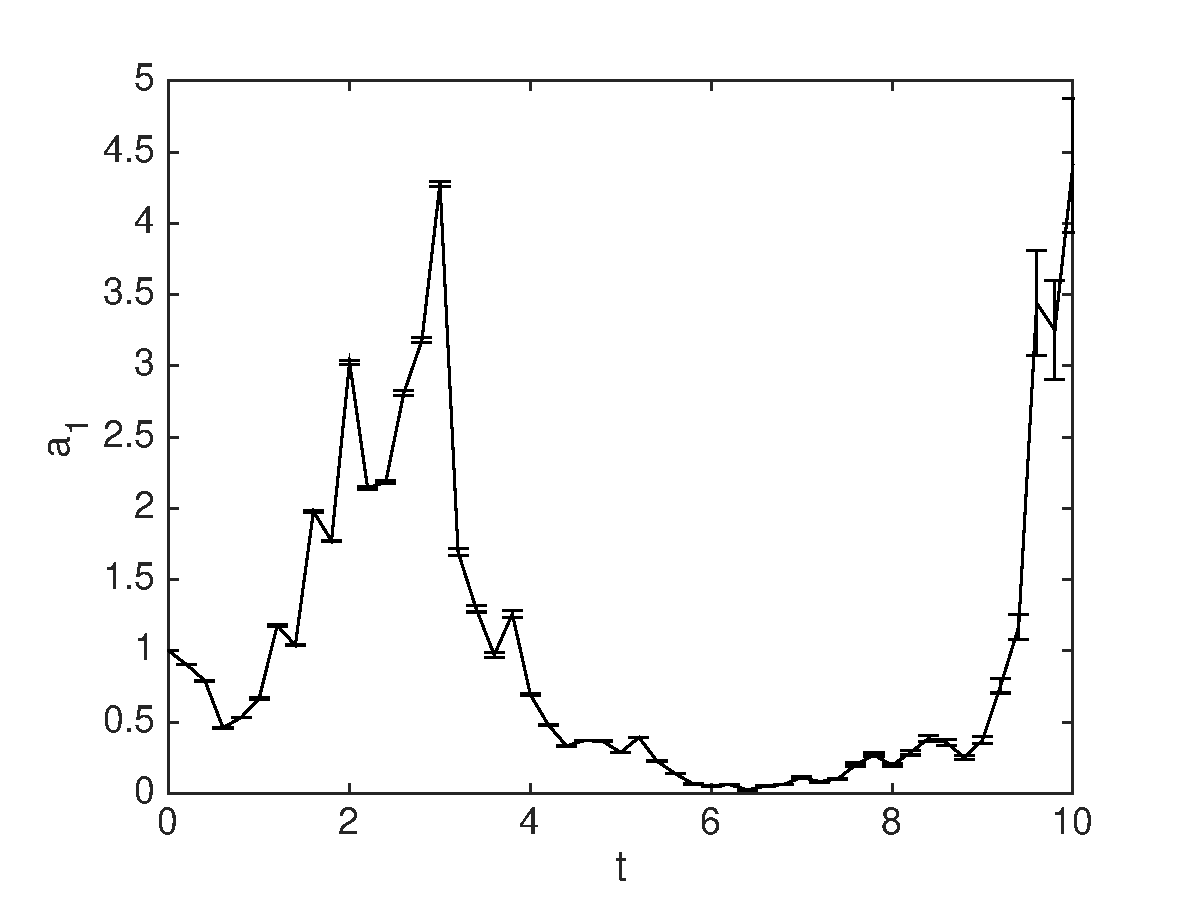
\includegraphics[width=0.75\textwidth]{Figures/Black-Scholes}\caption{\label{fig:The-Black-Scholes}Simulation of the Black-Scholes equation
describing stock prices.}
\end{figure}

Note that $in.initial$ describes the initialization function. The
first argument of $@(v,r)$ is $v$, an initial random variable with
unit variance. The error-bars are estimates of step-size error. Errors
can be reduced by using more time-steps.
\begin{itemize}
\item \textbf{Solve for a more mature stock having $\mu=0.1,\,\sigma=0.1$.}
\end{itemize}

\chapter{xSPDE Projects \label{chap:Projects-xSPDE}}

Projects are larger scale investigations, where files are used to
record inputs and data. This requires a new input parameter:

\begin{center}
\begin{tabular}{|c|c|c|c|}
\hline 
Label  & Type  & Default value  & Description\tabularnewline
\hline 
\hline 
\emph{in.file}  & string  & \emph{''}  & Matlab or HDF5 data file\tabularnewline
\hline 
\end{tabular}
\par\end{center}

\section{Ensembles and sampling errors}

Averages over stochastic ensembles are the specialty of xSPDE, which
requires specification of the ensemble size. A sophisticated hierarchy
of ensemble specifications in three levels is possible, to allow maximum
resource utilization, so that:
\[
in.ensembles=[ensembles(1),ensembles(2),ensembles(3)]\,.
\]
The local ensemble, $ensembles\left(1\right)$, gives within-thread
parallelism, allowing vector instruction use for single-core efficiency.
The serial ensemble, $ensembles\left(2\right)$, gives a number of
independent trajectories calculated serially. 

The parallel ensemble, $ensembles\left(3\right)$, gives multi-core
parallelism, and requires the Matlab parallel toolbox. This improves
speed when there are multiple cores. One should optimally put $ensembles\left(3\right)$
equal to the available number of CPU cores.

The \emph{total }number of stochastic trajectories or samples is 
\[
ensembles(1)\times ensembles(2)\times ensembles(3)\,.
\]

Either $ensembles(2)$ or $ensembles(3)$ are required if sampling
error-bars are to be calculated, owing to the sub-ensemble averaging
method used in xSPDE to calculate sampling errors accurately. 

\section{xSIM and xGRAPH}

An XPDE session can either run simulations interactively, described
in Chapter \ref{chap:Interactive-xSPDE}, or else using a function
file called a project file. This allows xSPDE to run in a batch mode,
as needed for longer projects which involve large ensembles. In either
case, the Matlab path must include the xSPDE folder. For generating
graphs automatically, the script input or project function should
end with the combined function \textbf{xspde(in)}. 

With batch jobs it is often useful to divide xSPDE into its simulation
function, xSIM, and its graphics function, xGRAPH, to allow graphs
to be made at a later time from the simulation. In this case the function\textbf{
$xsim$} runs the simulation, and $xgraph$ makes the graphs. The
two-stage option is better for running batch jobs, which you can graph
at a later time.

To create a data file, you must enter the filename when running the
simulation, using the $in.file=filename$ input. A typical xSPDE project
function of this type is as follows:

\begin{eqnarray*}
\mathtt{function}\,[e,ec] & = & project.m\\
\mathtt{in.}[label1] & = & [parameter1]\\
\mathtt{in.}[label2] & = & \ldots\\
\mathtt{in.file} & = & [my\,file].\mathtt{mat}\\
\mathtt{[e,in]} & = & \mathtt{xsim(in)}\\
\mathtt{ec} & = & \mathtt{xgraph(in.file)}\\
\mathtt{end}
\end{eqnarray*}

After preparing a project file using the editor, click on the Run
arrow above the editor window. 

In summary, a simple batch job workflow is as follows:
\begin{itemize}
\item Create the metadata $in$, and include a file name
\item Change the Matlab directory path to home using $cd\,\sim$.
\item Run the simulation with\textbf{ {[}e,in{]}=xsim(in)}.
\item Note that xSIM changes the file-name if it already exists, and returns
the new name for plotting.
\item Run \textbf{xgraph(in.file)}, and the data will be accessed and graphed. 
\item You can use either Matlab (.mat) or standard HDF5 (.h5) file-types.
\end{itemize}

\section{Kubo project}

To get started on more complex programs, we next simulate the Kubo
oscillator, which is an oscillator with a random frequency: 
\begin{equation}
\dot{a}=iaw
\end{equation}

\subsection*{Exercises}
\begin{itemize}
\item \textbf{Simulate the Kubo oscillator using a file, $Kubo.m$, with
two ensembles to allow sampling error estimates. The error vector
$error$ gives the time-step error plus the sampling error.}
\end{itemize}
\begin{center}
\noindent\doublebox{\begin{minipage}[t]{1\columnwidth - 2\fboxsep - 7.5\fboxrule - 1pt}%
\texttt{function {[}error{]} = Kubo() }

\texttt{in.name = 'Kubo oscillator';}

\texttt{in.ensembles = {[}400,16{]}; }

\texttt{in.initial = @(v,r) 1+0{*}v;}

\texttt{in.da = @(a,w,r) i{*}a.{*}w;}

\texttt{in.olabels = '\textless{}a\_1\textgreater{}';}

\texttt{in.file = 'kubo.mat';}

\texttt{{[}error,in{]}=xsim(in); }

\texttt{xgraph(in.file);}

\texttt{end}%
\end{minipage}}
\par\end{center}

The initial value of 1 is modified by adding $0*v$. This is necessary,
so that it returns an array whose first dimension equals the ensemble
size. 

This function is designed to generate a data file, \texttt{kubo.mat}.
If you run this more than once without deleting the earlier file,
you will get a warning and a new file-name, \texttt{kubo1.mat}, which
is stored in the in structure. Under these circumstance, xgraph will
graph the data in the most recent file saved, with the new file-name.
This occurs because xSPDE will \textbf{not} overwrite old files, to
protect your previous data. 

You can also include modified graphics parameters as a second input
when running \texttt{xgraph, }just in case the first graphs you generate
need changes.

\section{Open system}

We next simulate the driven quantum oscillator with a vacuum noise
input and output
\begin{equation}
\dot{a}=iaw
\end{equation}

\subsection*{Exercises}
\begin{itemize}
\item \textbf{Simulate the Kubo oscillator using a file, $Kubo.m$, with
two ensembles to allow sampling error estimates. The error vector
$error$ gives the time-step error plus the sampling error.}
\end{itemize}
\begin{center}
\noindent\doublebox{\begin{minipage}[t]{1\columnwidth - 2\fboxsep - 7.5\fboxrule - 1pt}%
\texttt{function {[}error{]} = Kubo() }

\texttt{in.name = 'Kubo oscillator';}

\texttt{in.ensembles = {[}400,16{]}; }

\texttt{in.initial = @(v,r) 1+0{*}v;}

\texttt{in.da = @(a,w,r) i{*}a.{*}w;}

\texttt{in.olabels = '\textless{}a\_1\textgreater{}';}

\texttt{in.file = 'kubo.mat';}

\texttt{{[}error,in{]}=xsim(in); }

\texttt{xgraph(in.file);}

\texttt{end}%
\end{minipage}}
\par\end{center}

The initial value of 1 is modified by adding $0*v$. This is necessary,
so that it returns an array whose first dimension equals the ensemble
size. 

This function is designed to generate a data file, \texttt{kubo.mat}.
If you run this more than once without deleting the earlier file,
you will get a warning and a new file-name, \texttt{kubo1.mat}, which
is stored in the in structure. Under these circumstance, xgraph will
graph the data in the most recent file saved, with the new file-name.
This occurs because xSPDE will \textbf{not} overwrite old files, to
protect your previous data. 

You can also include modified graphics parameters as a second input
when running \texttt{xgraph, }just in case the first graphs you generate
need changes.

\section{Challenge problem \#1}

This is a much harder example, involving a full nonlinear quantum
phase-space simulation. The method can also be used to investigate
quantum non-equilibrium phase transitions, tunneling in open systems,
quantum entanglement, Einstein-Podolsky-Rosen paradoxes, Bell violations,
and many other problems treated in the literature\cite{Gardiner,Drummond}.

The following new ideas are introduced: 
\begin{enumerate}
\item \textbf{$\mathtt{in.ranges}$ is the space-time integration range.} 
\item \textbf{$\mathtt{in.steps}$ gives integration steps per plot-point,
for accuracy.} 
\end{enumerate}
A simple case is the nonlinear driven quantum oscillator - for example,
an optomechanical, atomic or nonlinear optical medium in a driven
cavity. 

The phase-space Fokker-Planck equation is equivalent to an SDE with
the following form 
\begin{eqnarray}
\frac{d\alpha}{dt} & = & -\tilde{\gamma}\alpha-i\kappa\alpha^{2}\beta+\mathcal{E}+i\sqrt{i\kappa}\alpha w_{1}(t),\nonumber \\
\frac{d\beta}{dt} & = & -\tilde{\gamma}^{\ast}\beta+i\kappa\beta^{2}\alpha+\mathcal{E}^{\ast}+\sqrt{i\kappa}\beta w_{2}(t),
\end{eqnarray}
where $\xi_{i}(t)$ are independent Gaussian noise terms with zero
means and the following nonzero correlations 
\begin{equation}
\left\langle w_{i}(t)w_{j}(t^{\prime})\right\rangle =\delta_{ij}\delta(t-t^{\prime}).
\end{equation}

Note that these equations require that $\kappa\ll\gamma$, which is
typical experimentally, otherwise one must use additional stochastic
gauge stabilization to improve sampling error. 

Defining the dimensionless parameters $\varepsilon$ and $\lambda$
as 
\begin{equation}
\varepsilon=\frac{2\mathcal{E}}{\kappa}\,,\;\lambda=\frac{2\tilde{\gamma}}{\kappa}\,\,.\label{parameters}
\end{equation}
Provided $\gamma+\Delta\omega<0$ and $($Re$\lambda)^{2}>3|\lambda|^{2}$
there is a bistable region. This means that for $|\varepsilon|^{2}$
in a certain range, there are two physically possible values of $n_{0}$.
For $\tilde{\gamma}=2.5-10i$, $\kappa=1$, the bistable region is
around $\mathcal{E}=8$. The observed quantity is the particle number,
$\left\langle \hat{a}^{\dagger}\hat{a}\right\rangle =\left\langle \alpha\beta\right\rangle $,
with stable values of $n\approx1$ and $n\approx6$. 

\subsection*{Exercises}
\begin{itemize}
\item \textbf{Simulate the nonlinear oscillator by creating a file, $Nonlinear.m$ }
\item \textbf{Can you observe quantum tunneling of $n=\alpha\beta$ in the
bistable regime?}
\item \textbf{Do you see transient Schroedinger `cat states' with a negative
n value?}
\end{itemize}
Since tunneling is random, for real experimental comparisons, one
would have to measure correlation functions and spectra. However,
a tunneling event in a simulation indicates that it is likely in experiment
too. These calculations require long time scales, $\mathtt{in.ranges}$,
to observe tunneling, and a large number of time steps per plotted
point, $\mathtt{in.steps}$, to maintain accuracy in the quantum simulations.

\chapter{Stochastic PDEs\label{chap:Stochastic-partial-differential}}

A stochastic partial differential equation or $SPDE$ for a complex
vector field is defined in both time $t$ and space dimensions $\bm{x}$.
The total \emph{dimension} $d$ in xSPDE is unlimited, and includes
time and space. Large $d$ is memory-intensive and slow! The general
equation solved can be written in differential form as

\begin{equation}
\frac{\partial\mathbf{a}}{\partial t}=\mathbf{A}\left[\mathbf{a}\right]+\underline{\mathbf{B}}\left[\mathbf{a}\right]\cdot\bm{w}(t)+\underline{\mathbf{L}}\left[\bm{\nabla}\right]\cdot\mathbf{a}\,.
\end{equation}
Here $\mathbf{a}$ is a real or complex vector or vector field. The
\emph{initial} conditions are arbitrary functions. $\mathbf{A}\left[\mathbf{a}\right]$
and $\underline{\mathbf{B}}\left[\mathbf{a}\right]$ are vector and
matrix functions of $\mathbf{a}$, $\underline{\mathbf{L}}\left[\bm{\nabla}\right]$
is a matrix of \emph{linear} terms including derivatives, diagonal
in the vector indices, and $\mathbf{w}=\left[\bm{w}^{x},\bm{w}^{k}\right]$
are real delta-correlated noise fields such that: 
\begin{eqnarray}
\left\langle w_{i}^{x}\left(t,\bm{x}\right)w_{j}^{x}\left(t,\bm{x}'\right)\right\rangle  & = & \delta\left(\bm{x}-\bm{x}'\right)\delta\left(t-t'\right)\delta_{ij}\nonumber \\
\left\langle w_{i}^{k}\left(t,\bm{k}\right)w_{j}^{k}\left(t,\bm{k}'\right)\right\rangle  & = & f(\mathbf{k})\delta\left(\bm{k}-\bm{k}'\right)\delta\left(t-t'\right)\delta_{ij}.
\end{eqnarray}

Transverse \emph{boundaries} are of three types: Neumann (vanishing
derivative), periodic, or Dirichlet (vanishing field). These are indicated
using $boundaries=-1,0,1$. The term $\underline{\mathbf{L}}\left[\bm{\nabla}\right]$
may be omitted if $d=1$, as there are no space dimensions. Here $f(\mathbf{k})$
is an arbitrary momentum filter, for correlated noise. The linear
function $L$ is input as a separate function in xSPDE, to allow for
greatest efficiency and use of an interaction picture. Note that it
depends on momentum space coordinates, and this involves Fourier transforms.

\section{Coordinates and boundary conditions}

The spatial interval used is from a preset \emph{origin} $\bm{o}$,
and has predetermined \emph{ranges} $\mathbf{r}$. In the x-dimension,
the problem is solved on a transverse interval of $x=[o_{2},o_{2}+r_{2}]$.
Note that all dimensions are numbered starting with the time dimension
as $i=1$. In order to discretize the problem for solution the $n_{i}$
lattice \emph{points} are fitted into the spatial interval so that
$dx_{i}=r_{i}/(n_{i}-1)$, ie:
\begin{equation}
x_{i}=o_{i}+(n_{i}-1)dx_{i}\,.
\end{equation}

The default boundary conditions are periodic. Otherwise, details of
boundaries are as follows:
\begin{description}
\item [{Neumann:}] For vanishing \emph{derivative} boundaries, use $in.boundaries=-1$
\item [{Periodic:}] For periodic boundaries - which is the default case
- use $in.boundaries=0$
\item [{Dirichlet:}] For vanishing \emph{field} boundaries, $in.boundaries=1$
\end{description}
These are specified independently in different columns for each dimension
- starting with time for consistency - and in different rows for the
lower and upper coordinate boundary, such as $[0,1,1;0,1,1]$. Note
that in current versions of xspde, the equations are always initial
value problems, so the first dimension specification is not used.
The default option is periodic boundaries if $in.boundaries$ is not
specified. For other types of nonvanishing specified boundary conditions,
it is recommended that auxiliary fields are used, whose value must
be added to the standard field.

The xSPDE spectral definition in space-time is:
\begin{equation}
\tilde{a}(\omega,\bm{k})=\frac{1}{\left[2\pi\right]^{d/2}}\int e^{i(\bm{k}\cdot\bm{x}-\omega t)}a(t,\bm{x})dtd\bm{x}\,
\end{equation}

This is translated into a sum over the lattice points using a discrete
Fourier transform at the lattice points $x_{i}$, so that: 

\begin{equation}
\tilde{a}(\omega_{i},\bm{k}_{i})=\frac{dtd\mathbf{x}}{\left[2\pi\right]^{d/2}}\sum_{j_{1}\ldots j_{d}}\exp\left[i\left(\bm{k}_{\bm{i}}\cdot\bm{x}_{\bm{j}}-\omega_{i_{1}}t_{j_{1}}\right)\right]a(t_{j_{1}},\bm{x}_{\bm{j}})\,
\end{equation}
The momenta $k_{i}$ have an interval of
\begin{equation}
dk_{i}=\frac{2\pi}{n_{i}dx_{i}}
\end{equation}
with $k_{i}$ values given for even n by: 
\begin{equation}
k_{i}=\left(1-\frac{n_{i}}{2}\right)dk_{i},\ldots\frac{n_{i}}{2}dk_{i}
\end{equation}
and for odd n by:
\begin{equation}
k_{i}=\frac{1-n_{i}}{2}dk_{i},\ldots\frac{n_{i}-1}{2}dk_{i}
\end{equation}

\begin{equation}
k_{i}=\frac{1-n_{i}}{2}dk_{i},\ldots\frac{n_{i}-1}{2}dk_{i}
\end{equation}

\section{Stochastic Ginzburg-Landau equation}

Including space-time dimensions with $d=3$, an example of a SPDE
is the stochastic Ginzburg-Landau equation. This describes symmetry
breaking: the system develops a spontaneous phase which can vary spatially
as well. The model is widely used to describe lasers, magnetism, superconductivity,
superfluidity and even particle physics: 
\begin{equation}
\dot{a}=\left(1-\left|a\right|^{2}\right)a+bw(t)+c\nabla^{2}a
\end{equation}
where 
\begin{equation}
\left\langle w(x)w^{*}(x')\right\rangle =2\delta\left(t-t'\right)\delta\left(x-x'\right).
\end{equation}

The following new ideas are introduced for this problem: 
\begin{enumerate}
\item \textbf{$\mathtt{in.dimension}$ is the space-time dimension.} 
\item \textbf{The} 'dot' \textbf{notation used for parallel operations over
lattices}.
\item \textbf{$\mathtt{in.linear}$ is the linear operator - a laplacian
in these cases.}
\item \textbf{$\mathtt{in.images}$ produces movie-style images at discrete
time slices.}
\item \textbf{$\mathtt{r.Dx}$ indicates a derivative operation, $\partial/\partial x$.} 
\item \textbf{$-5<x<5$ is the default xSPDE coordinate range in space.} 
\end{enumerate}

\subsection*{Exercises}
\begin{itemize}
\item \textbf{Solve the stochastic G-L equation for $b=0.001$ and $c=0.01i$.}
\item \textbf{Change to a real diffusion so that $c=0.1$.}
\end{itemize}
In the first case, you should get the output graphed in Fig (\ref{fig:Symmetry-breaking})
.

\begin{center}
\noindent\doublebox{\begin{minipage}[t]{1\columnwidth - 2\fboxsep - 7.5\fboxrule - 1pt}%
\texttt{in.noises=2;}

\texttt{in.dimension=3;}

\texttt{in.steps=10;}

\texttt{in.linear = @(r) i{*}0.01{*}(r.Dx.\textasciicircum{}2+r.Dy.\textasciicircum{}2);}

\texttt{in.observe = @(a,\textasciitilde{}) abs(a).\textasciicircum{}2;}

\texttt{in.images =6;}

\texttt{in.olabels = '\textbar{}a\textbar{}\textasciicircum{}2';}

\texttt{in.da=@(a,w,\textasciitilde{}) (1-abs(a(1,:)).\textasciicircum{}2).{*}a+0.001{*}(w(1,:)+i{*}w(2,:));}

\texttt{xspde(in)}%
\end{minipage}}
\par\end{center}

Here the notation $z(1,:)$ is like the dot: the colon means that
the operation is repeated over all values of the second index, which
is the spatial lattice index.

\begin{figure}
\centering{}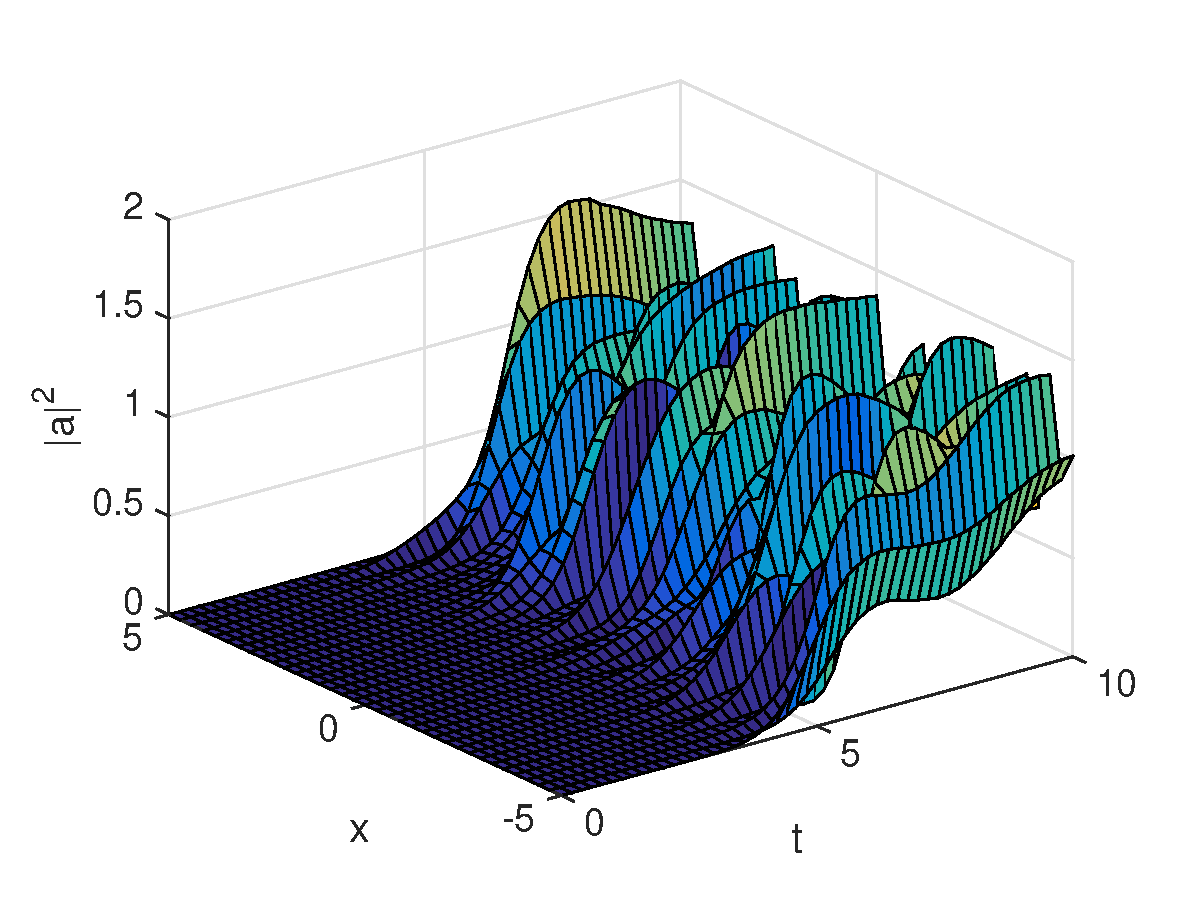
\includegraphics[width=0.75\textwidth]{Figures/GinzLand}\caption{\label{fig:Symmetry-breaking}Simulation of the stochastic equation
describing symmetry breaking in two dimensions. Spatial fluctuations
are caused by the different phase-domains that interfere. The graph
obtained here is projected onto the $y=0$ plane. }
\end{figure}

\section{Soliton}

The famous nonlinear Schr�dinger equation (NLSE) is: 
\[
\frac{da}{dt}=\frac{i}{2}\left[\nabla^{2}a-a\right]+ia\left|a\right|^{2}
\]

Together with the initial condition that $a(0,x)=sech(x)$, this has
a soliton, an exact solution that doesn't change in time: 
\begin{eqnarray*}
a(t,x) & = & sech(x)
\end{eqnarray*}
The Fourier transform at $k=0$ is simply: 
\begin{eqnarray*}
\tilde{a}(t,0) & = & \frac{1}{\sqrt{2\pi}}\int sech(x)dx=\sqrt{\frac{\pi}{2}}
\end{eqnarray*}

\subsection*{Exercises}
\begin{itemize}
\item \textbf{Solve the NLSE for a soliton}
\end{itemize}
\begin{center}
\noindent\doublebox{\begin{minipage}[t]{1\columnwidth - 2\fboxsep - 7.5\fboxrule - 1pt}%
f\texttt{unction {[}e{]} = Soliton() }

\texttt{in.name = 'NLS soliton';}

\texttt{in.dimension = 2; }

\texttt{in.initial = @(v,r) sech(r.x); }

\texttt{in.da = @(a,\textasciitilde{},r) i{*}a.{*}(conj(a).{*}a);}

\texttt{in.linear = @(r) 0.5{*}i{*}(r.Dx.\textasciicircum{}2-1.0);}

\texttt{in.olabels = \{'a\_1(x)'\}; }

\texttt{in.compare\{1\}= @(t,\textasciitilde{}) 1; }

\texttt{e = xspde(in); }

\texttt{end}%
\end{minipage}} 
\par\end{center}
\begin{itemize}
\item \textbf{Add an additive complex noise of $0.01(w_{1}+iw_{2}$) to
the differential equation, then replot with an average over $1000$
samples.}
\end{itemize}
\newpage{}

\section{Gaussian diffraction }

Free diffraction of a Gaussian wave-function in three dimensions,
is given by 
\[
\frac{da}{dt}=\frac{i}{2}\nabla^{2}a
\]

The xSPDE spectral definition in space-time is:
\[
\tilde{a}(\omega,\bm{k})=\frac{1}{\left[2\pi\right]^{d/2}}\int e^{i(\bm{k}\cdot\bm{x}-\omega t)}a(t,\bm{x})dtd\bm{x}\,
\]

Together with the initial condition that $a(0,x)=exp(-\left|\mathbf{x}\right|^{2}/2)$,
this has an exact solution for the diffracted intensity in either
ordinary space or momentum space is therefore: 
\begin{eqnarray*}
\left|a\left(t,\mathbf{x}\right)\right|^{2} & = & \frac{1}{\left(1+t^{2}\right)^{3/2}}exp(-\left|\mathbf{x}\right|^{2}/\left(1+t^{2}\right))\\
\left|\tilde{a}\left(t,\mathbf{k}\right)\right|^{2} & = & exp(-\left|\mathbf{k}\right|^{2})
\end{eqnarray*}

To get an output from a spatially fourier transformed field in three-dimensions,
but without a fourier transform in time, just set $in.transforms=[0,1,1,1]$,
for the particular observable you need to calculate in transform space.

\subsection*{Exercises}
\begin{itemize}
\item \textbf{Solve the diffraction equation without noise}
\item Note that the example below stores data in a standardized HDF5 file.
\end{itemize}
\begin{center}
\noindent\doublebox{\begin{minipage}[t]{1\columnwidth - 2\fboxsep - 7.5\fboxrule - 1pt}%
\texttt{function {[}e{]} = Gaussian() }

\texttt{in.dimension = 4; }

\texttt{in.initial = @(v,r) exp(-0.5{*}(r.x.\textasciicircum{}2+r.y.\textasciicircum{}2+r.z.\textasciicircum{}2));}

\texttt{in.linear = @(r) 1i{*}0.05{*}(r.Dx.\textasciicircum{}2+r.Dy.\textasciicircum{}2+r.Dz.\textasciicircum{}2); }

\texttt{in.observe = @(a,r) a.{*}conj(a); }

\texttt{in.olabels = '\textbar{}a(x)\textbar{}\textasciicircum{}2'; }

\texttt{in.file = 'Gaussian.h5';}

\texttt{in.images = 4;}

\texttt{{[}e,in{]} = xsim(in); }

\texttt{e = xgraph(in.file); }

\texttt{end } %
\end{minipage}}
\par\end{center}
\begin{itemize}
\item \textbf{Add an additive complex noise of $0.01(w_{1}+iw_{2}$) to
the Gaussian differential equation, then replot with an average over
$10$ samples.}
\end{itemize}
Note that for this, you'll need to define $in.da=@(a,w,r)0.01*(w(1,:)+i*w(2,:))$

\newpage{}

\section{Planar noise}

The next example is growth of thermal noise of a two-component complex
field in a plane, given by the equation 
\[
\frac{d\bm{a}}{dt}=\frac{i}{2}\nabla^{2}\bm{a}+\bm{w}(t,x)
\]
where $\bm{\zeta}$ is a delta-correlated complex noise vector field:
\[
w_{j}(t,\mathbf{x})=\left[w_{j}^{re}(t,\mathbf{x})+i\zeta_{j}^{im}(t,\mathbf{x})\right]/\sqrt{2},
\]
with the initial condition that the initial noise is delta-correlated
in position space 
\[
a(0,\mathbf{x})=\bm{\zeta}^{(in)}(\bm{x})
\]
where: 
\[
\bm{\zeta}^{(in)}(\bm{x})=\left[\bm{\zeta}^{re(in)}(\mathbf{x})+i\bm{\zeta}^{im(in)}(\mathbf{x})\right]/\sqrt{2}
\]

This has an exact solution for the noise intensity in either ordinary
space or momentum space: 
\begin{eqnarray*}
\left\langle \left|a_{j}\left(t,\mathbf{x}\right)\right|^{2}\right\rangle  & = & (1+t)/dV\\
\left\langle \left|\tilde{a}_{j}\left(t,\mathbf{k}\right)\right|^{2}\right\rangle  & = & (1+t)/dV_{k}\\
\left\langle \tilde{a}_{1}\left(t,\mathbf{k}\right)\tilde{a}_{2}^{*}\left(t,\mathbf{k}\right)\right\rangle  & = & 0
\end{eqnarray*}

Here, the noise is delta-correlated, and $dV$, $dV_{k}$ are the
cartesian space and momentum space lattice cell volumes respectively.
Suppose that $n=n_{x}n_{y}$ is the total number of spatial points,
and there are $n_{x(y)}$ points in the x(y)-direction, so then: 
\begin{eqnarray*}
dV & = & dxdy\\
dV_{k} & = & dk_{x}dk_{y}=\frac{(2\pi)^{2}}{ndV}.
\end{eqnarray*}

In the simulations, two planar noise fields are propagated, one using
delta-correlated noise, the other with noise transformed to momentum
space to allow filtering. This allows use of finite correlation lengths
when needed, by including a frequency filter function that is used
to multiply the noise in Fourier-space. The Fourier-space noise variance
is the square of the filter function. 

The first noise index, $in.noises(1)$, indicates how many noise fields
are generated, while $in.noises(2)$ indicates how many of these are
spatially correlated, via Fourier transform, filter and inverse Fourier
transform. These appear to the user as additional noises, so the total
is $in.noises(1)+in.noises(2)$. The filtered noises have a finite
correlation length. They are correlated with the first $in.noises(1)$
x-space noises they are generated from, as this can be useful. 

\subsection*{Exercises}
\begin{itemize}
\item \textbf{Solve the planar noise growth equation}
\end{itemize}
\begin{center}
\noindent\doublebox{\begin{minipage}[t]{1\columnwidth - 2\fboxsep - 7.5\fboxrule - 1pt}%
\texttt{function {[}e{]} = Planar() }

\texttt{in.name = 'Planar noise growth'; }

\texttt{in.dimension = 3; }

\texttt{in.fields = 2; }

\texttt{in.ranges = {[}1,5,5{]}; }

\texttt{in.steps = 2; }

\texttt{in.noises = {[}4,2{]}; }

\texttt{in.ensembles = {[}10,4,4{]}; }

\texttt{in.initial = @Initial; }

\texttt{in.da = @Da; }

\texttt{in.linear = @Linear; }

\texttt{in.observe = @(a,r) a(1,:).{*}conj(a(1,:));}

\texttt{in.olabels= '\textless{}\textbar{}a\_1(x)\textbar{}\textasciicircum{}2\textgreater{}';}

\texttt{in.compare = @(t,in) {[}1+t{]}/in.dV;}

\texttt{in.images = 4; }

\texttt{e = xspde(in); }

\texttt{end }\\
 \texttt{ }

\texttt{function a0 = Initial(v,r) }

\texttt{a0(1,:) = (v(5,:)+1i{*}v(6,:))/sqrt(2); }

\texttt{a0(2,:) = (v(3,:)+1i{*}v(4,:))/sqrt(2); }

\texttt{end }\\
\texttt{ }

\texttt{function da = Da(a,z,r) }

\texttt{da(1,:) = (z(5,:)+1i{*}z(6,:))/sqrt(2); }

\texttt{da(2,:) = (z(3,:)+1i{*}z(4,:))/sqrt(2); }

\texttt{end }\\
 \texttt{ }

\texttt{function L = Linear(r) }

\texttt{lap = r.Dx.\textasciicircum{}2+r.Dy.\textasciicircum{}2; }

\texttt{L(1,:) = 1i{*}0.5{*}lap(:); }

\texttt{L(2,:) = 1i{*}0.5{*}lap(:); }

\texttt{end}%
\end{minipage}} 
\par\end{center}
\begin{itemize}
\item \textbf{Add a decay rate of $-a$ to the differential equation, then
replot}
\item \textbf{Add growth and nonlinear saturation terms}
\end{itemize}
\newpage{}

\section{Characteristic equation}

The next example is the characteristic equation for a traveling wave
at constant velocity. It is included to illustrate what happens at
periodic boundaries, when Fourier-transform methods are used for propagation.
There are a number of methods known to prevent this effect, including
addition of absorbers - often called apodization - at the boundaries.
The equation is: 
\[
\frac{da}{dt}+\frac{da}{dx}=0
\]

Together with the initial condition that $a(0,x)=sech(2x+5)$, this
has an exact solution that propagates at a constant velocity: 
\begin{eqnarray*}
a(t,x) & = & sech(2(x-t)+5)
\end{eqnarray*}
The time evolution at $x=0$ is simply: 
\begin{eqnarray*}
a(t,0) & = & sech(2(t-5/2))
\end{eqnarray*}

\subsection*{Exercises}
\begin{itemize}
\item \textbf{Solve the characteristic equation given above, noting the
effects of periodic boundaries.}
\end{itemize}
\begin{center}
\noindent\doublebox{\begin{minipage}[t]{1\columnwidth - 2\fboxsep - 7.5\fboxrule - 1pt}%
\texttt{function {[}e{]} = Characteristic() }

\texttt{in.name = 'Characteristic'}

\texttt{in.dimension = 2; }

\texttt{in.initial = @(v,r) sech(2.{*}(r.x+2.5)); }

\texttt{in.da = @(a,z,r) 0{*}a; }

\texttt{in.linear = @(r) -r.Dx; }

\texttt{in.olabels = 'a\_1(x)'; }

\texttt{in.compare = @(t,in) sech(2.{*}(t-2.5)); }

\texttt{e = xspde(in); }

\texttt{end }%
\end{minipage}} 
\par\end{center}
\begin{itemize}
\item \textbf{Recalculate with the opposite velocity, and a new exact solution.}
\end{itemize}

\section{Challenge problem \#2}

Counter-intuitively, a random potential \emph{prevents} normal wave-packet
spreading in quantum-mechanics. This is Anderson localization: a famous
property of quantum mechanics in a random potential. A typical experimental
method is to confine an ultra-cold Bose-Einstein condensate (BEC)
in a trap, then release the BEC in a random external potential produced
by a laser. The expansion rate of the BEC is reduced by the Anderson
localization due to the random potential. Physically, the observable
quantity is the particle density $n=\left|\psi\right|^{2}$.

This can be treated either using a Schroedinger equation with a random
potential, at low density, or using the Gross-Pitaevskii (GP) equation
to include atom-atom interactions at the mean field level. In this
example of a problem where strong localization occurs, the general
equations are: 

\[
\frac{\partial\psi}{\partial t}=\frac{1}{i\hbar}\left[-\frac{\hbar^{2}}{2m}\nabla^{2}+V\left(\bm{r}\right)+g\left|\psi\right|^{2}\right]\psi
\]

In calculations, it is best to use a dimensionless form by rescaling
coordinates and fields. A simple way to simulate this with xSPDE is
to treat $\psi$ as a scaled field $a(1),$ and to assume the random
potential field $V\left(\bm{r}\right)$ as caused by interactions
with second random field $\left|a(2)\right|^{2}$. This has the advantage
that it is similar to the actual experiment, and allows one to treat
time-dependent potentials as well, if desired. 

With the rescaling, this simplifies to:
\[
\frac{\partial a_{1}}{\partial\tau}=i\left[\frac{\partial}{\partial\zeta^{2}}^{2}-\left|a_{2}\right|^{2}-\left|a_{1}\right|^{2}\right]a_{1}
\]

A convenient initial condition is to use: 
\begin{eqnarray*}
a_{1} & = & a_{0}\exp(-\zeta^{2})\\
\left\langle a_{2}(\zeta)a_{2}(\zeta')\right\rangle  & = & v\delta\left(\zeta-\zeta'\right)
\end{eqnarray*}

\subsection*{Exercise}
\begin{itemize}
\item \textbf{Solve Schroedinger's equation without a random potential,
to observe expansion.}
\item \textbf{Include a random potential $v$, to observe localization.}
\item \textbf{Experiment with nonlinear terms and higher dimensions.}
\end{itemize}
Note that the GP equation is a mean field approximation; this is still
not a full solution of the many-body problem! Also, the experiments
are somewhat more complicated than this, and actually observe the
momentum distribution.

\chapter{Logic and data\label{chap:Logic-and-data}}

The simulation program logic is straightforward. It is a very compact
function called \textbf{xspde}. This calls \textbf{xsim},
for the simulation, then \textbf{xgraph} for the graphics. Most
of the work is done by other specialized functions. Input parameters
come from an \textbf{input} array, output is saved either in a \textbf{data}
array, or else in a specified file. During the simulation, global
averages and error-bars are calculated for both time-step and sampling
errors. When completed, timing and error results are printed. 

\section{Simulation function, \emph{xsim}}

\subsection{Input and data structures}

To explain xSPDE in full detail, 
\begin{itemize}
\item Simulation inputs are stored in the \textbf{input} cell array. 
\item This describes a \emph{sequence} of simulations, so that \textbf{input=\{in1,in2,...\}}. 
\item Each structure \textbf{in} describes a simulation, whose output is
the input of the next. 
\item The main simulation function is called using $\mathbf{xsim(input)}$. 
\item Averages are recorded sequentially in the \textbf{data} cell array. 
\item Raw trajectory data is stored in the \textbf{raw} cell array if required. 
\end{itemize}
The sequence $\mathbf{input}$ has a number of individual simulation
objects $\mathbf{in}$. Each includes parameters that specify the
simulation, with functions that give the equations and observables.
If there is only one simulation, just one individual specification
$\mathbf{in}$ is needed. In addition, xSPDE generates graphs with
its own graphics program.

\subsection{User definable simulation functions}

The most commonly used functions are indicated with an asterisk. Others
have automatic defaults that are not usually changed, except in special
cases.
\begin{description}
\item [{{*}initial}] is used to initialize each integration in time. This
is a user-defined function, which can involve random numbers if there
is an initial probability distribution. This creates a stochastic
field on the lattice, called \textbf{\emph{a.}} The default is $\mathbf{xinitial}$,
which sets fields to zero. The returned first dimension should be
fields(1). 
\item [{{*}observe}] is the initial observation function, whose output
is averaged over the ensembles, called from \textbf{xpath}. The default,
$\mathbf{xobserve}$, returns the real part of the amplitudes. 
\item [{{*}function}] is an optional function used to take arbitrary transforms
of the initial observe outputs, after averaging over the \emph{first}
ensemble. The default returns the averages unchanged. 
\item [{{*}linear}] is the linear response, including transverse derivatives
in space. The default, $\mathbf{xlinear}$, sets this to zero. 
\item [{{*}da}] is called by \textbf{step} to calculate derivatives of
the stochastic fields at every step in the process, including the
stochastic terms. The default, $\mathbf{xstep}$, sets this to zero.
The returned first dimension should be fields(1). All stochastic fields
are accessible as $a(n,:)$, where $n\leq fields(1)$.
\item [{{*}define}] is called by \textbf{step} to calculate any user-defined
auxiliary fields. The default, $\mathbf{xdefine}$, sets these to
zero. The returned first dimension should be fields(2). If auxiliary
fields are used they are accessible as $a(n,:)$, where $n>fields(1)$.
\item [{transfer}] is a function used to initialize sequential simulations,\textbf{
}where previous or output stochastic field values are automatically
included as input to the next stage ine the intergation sequence.
The default, $\mathbf{xtransfer}$, uses the output of the previous
simulation for the input to the next stage. This can be changed by
the user.
\item [{step}] is the algorithm that computes each step in time. This also
generates the random numbers at each time-step. Options include \textbf{xEuler},
\textbf{xRK2}, \textbf{xRK4, }for Euler and Runge-Kutta integration
methods. This can be user-modified by initializing the handle in.step
to add a new integration function. The default is $\mathbf{xRK4}$,
which is widely applicable. Another good option is$\mathbf{xMP}$,
which uses a midpoint or central-difference technique in the interaction
picture.
\item [{rfilter}] returns a momentum filter for random initial fields generated
in momentum space. The default, $\mathbf{xrfilter}$, sets this to
unity.
\item [{nfilter}] returns a momentum filter for random noises generated
in momentum space. The default, $\mathbf{xnfilter}$, sets this to
unity.
\item [{grid}] calculates the spatial integration grid. The default, $\mathbf{xgrid}$,
returns a rectangular grid in ordinary and momentum space.
\item [{prop}] is the spatial propagation function. The default, $\mathbf{xprop}$,
takes a Fourier transform of $\bm{a}$, multiplies by propfactor to
propagate in time, then takes an inverse Fourier transform. 
\item [{randomgen}] generates the initial random fields. The default, $\mathbf{xrandomgen}$,
returns Gaussian real fields that are delta-correlated in space or
momentum space.
\item [{noisegen}] generates the initial random fields. The default, $\mathbf{xnoisegen}$,
returns Gaussian real noises that are delta-correlated in time and
also in space or momentum space.
\item [{propfactor}] returns the interaction picture propagation factors.
The default, $\mathbf{xpropfactor}$, uses data from the $\mathbf{linear}$
function to calculate this.
\end{description}

\section{Arrays and errors}

Knowing the details of array indexing inside xSPDE isn't usually necessary.
Yet it becomes important if you want to write your own functions to
extend xSPDE, interface xSPDE with other functions, or read and write
xSPDE data files with external programs. It also helps to understand
how the program works.

\subsection{Array indexing}

In xSPDE, the space-time dimension $d$ is unlimited. All data, including
grid coordinates, fields and average results is stored in real or
complex numerical arrays of implicit or explicit rank $2+d$. During
the stochastic simulation, these arrays are flattened to matrices,
to shorten the Matlab code in the user functions. 

The index ordering is always $(i,\mathbf{j},e)$, where: 
\begin{itemize}
\item The first index is a field index ($i$). In some cases - like coordinates
- the first index is always $i=1$. 
\item The next $d$ indices $j_{1},\ldots j_{d}\equiv\bm{j}$ are for time
and space, where $\bm{j}$ indicates a $d$-dimensional index
\item The last index is an ensembles or checks index ($e/c$). For fields,
this is used to store field trajectories. For output data, it is used
to store means and error estimates.
\item To conserve memory, transient arrays during calculations use $\bm{j}=[1,j_{2},\ldots]$
, which indicates a $d$ dimensional index with time index set to
one. 
\end{itemize}
When the fields, noises or coordinates are integrated by the xSIM
integration functions, the field and data arrays are always flattened
to a matrix. This is for reasons of convenience in defining mathematical
operations. The first index is the field or line index, and the combined
second index covers all the rest: $(i,\mathbf{j},e)\rightarrow(i,J)$
This is done internally, but not in externally stored data, nor in
xGRAPH, which operates on the full data arrays.

Stored data uses heterogenous cell arrays to package numerical arrays
with additional high level indices. The first is always the sequence
index, $s$. Raw data also requires indices for checks and hih level
ensembles. Inside a sequence, data cell arrays have an additional
graph index $n$. This distinguishes the different averages generated
for output graphs and data. 

The following detailed information is not required to use xSPDE, but
it helps to give insight to how data is stored, and how to customize
and extend the code. There are several different types of arrays used.
These are as follows:
\begin{center}
\begin{tabular}{|c|c|c|}
\hline 
Label  & Indices  & Description\tabularnewline
\hline 
\hline 
\emph{a}  & $(i,\bm{j},e)$ & Stochastic fields\tabularnewline
\hline 
\emph{w}  & $(i,\bm{j},e)$ & Random and noise fields\tabularnewline
\hline 
\emph{x} & $(1,\bm{j},e)$ & Space coordinates\tabularnewline
\hline 
r & $\{s,c,f\}(i,\bm{j},e)$ & Raw data\tabularnewline
\hline 
o &  $\{n\}(o,\mathbf{j},c)$  & Observed average data\tabularnewline
\hline 
g & $\{s\}\{n\}(o,\mathbf{j},c)$  & Graph data\tabularnewline
\hline 
\end{tabular}
\par\end{center}

In summary, the xSPDE arrays are as follows:
\begin{itemize}
\item \textbf{Field} arrays $a(i,\bm{j},e)$ - these have a field index,
an ensemble index $e=1,\ldots ensembles(1)$, one time-point, and
a full spatial lattice.
\item \textbf{Random} and \textbf{noise} arrays $w(i,\bm{j},e)$ - these
are like field arrays. They are initial random fields or noise fields
for the stochastic equations. The first index can have a different
range to the field index.
\item \textbf{Coordinate} arrays $x(1,\bm{j},e)$ - these arrays are the
values of coordinates at grid-points, with labels $x,y,z$. Numeric
labels $x\{l\}$ are used with dimensions $d>4$, depending on the
axis number, $l=2,\ldots d$. The same sizes are used for: 
\begin{itemize}
\item momentum coordinates $kx,ky,kz$ (alternatively labelled $k\{2\},k\{3\},\ldots$)
- 
\item spectral derivative arrays $Dx,Dy,Dz$ (alternatively labelled $D\{2\},D\{3\},\ldots$)
.
\end{itemize}
\item \textbf{Raw} arrays $r\{s,c,f\}(i,\bm{j},e)$ These are like fields,
except with all time points stored. They are used optionally, as they
take up large amounts of memory. These are saved in cell arrays with
indices $s$ for the sequence, $c$ for the time-step check, $f$
for high-level ensemble index. 
\begin{itemize}
\item $s=1,\ldots S$ for the sequence number, 
\item $c=1,2$ for the error-checking time-step used, first coarse then
fine, 
\item $f=1,\ldots ensemble(2)*ensemble(3)$ for a high level combined parallel
and serial ensemble index.
\end{itemize}
\item \textbf{Data} arrays $d\{n\}(o,\mathbf{j},c)$ - these store the generated
average data at all time points, with an error-check index $c=1,2,3$.
Check indices are $c=1$ for the estimated average, $c=2$ for the
estimated time-step error, and $c=3$ for the estimated statistical
error or standard deviation. Note that the cell index $n$ is the
graph index, and the first array index $o$ is a user-generated graphics
line index. This may or may not correspond to a field index: it is
a user option.
\item \textbf{Graphics} data arrays $g\{s\}\{n\}(o,\mathbf{j},c))$ - these
store the complete sequence of \emph{data} that is plotted, and may
have further functional transformations when processed in \textbf{xgraph},
if required. Graphics cell data requires high-level cell indices $\{s\}$
for the sequence index, and $\{n\}$ for the graph or function index,
which corresponds to the index $\{n\}$ of the observe function used
to generate averages. One can have several data arrays to make a number
of distinct output graphs labelled $n$. Each graph may have multiple
averages, giving different liines for comparisons. These are then
combined into a sequence, each with different graphs, and therefore
need more indices. 
\end{itemize}
Although the indices always occur in the same order, the fields, noises
and output data can have different first dimensions. They are specified
using different input parameters. The output line index $o$ in a
graphics or data array describes different lines on a graph. Similarly,
the last ensemble index $e$ in a field array has a different range
to $c$, the check index, in a data array.

\subsection{Step-size errors}

Errors caused by the finite time-domain step-size, as well as those
caused by the finite ensemble, are checked automatically. Those caused
by the spatial lattice are not checked in the xSIM code. They must
be checked by manually, by comparing results with different transverse
lattice ranges and step-size.

Errors due to a finite step-size are estimated by comparing two simulations
with different step-sizes and the same random sequence, to make sure
the final results are accurate. The final 2D output graphs will have
error-bars if $checks=1$ was specified, which is also the default
parameter setting. Error-bars below a minimum relative size compared
to the vertical range of the plot, specified by the graphics variable
$minbar$, are not plotted. 

There is a clear strategy if the errors are too large. Either increase
the \emph{points}, which gives more plotted points and lower errors,
or increase the \emph{steps, }which reduces the step size without
changing the graphical resolution. The default algorithm and extrapolation
order can also be changed, please read the full xSPDE manual when
doing this. Error bars on the graphs can be removed by setting $checks=0$
or increasing $minbar$ in final graphs.

\subsection{Sampling errors}

Sampling error estimation in xSIM uses sub-ensemble averaging. This
generally leads to more reliable sampling error estimates, and makes
efficient use of the vector instruction sets that are used by Matlab.
Ensembles are specified in three levels. The first, \emph{ensemble(1)},
is called the number of samples for brevity. All computed quantities
returned by the \textbf{observe} functions are first averaged over
the samples, which are calculated efficiently using a parallel vector
of trajectories. By the central limit theorem, these low-level sample
averages are distributed as a normal distribution at large sample
number.

Next, the sample averages are averaged \textbf{again} over the two
higher level ensembles, if specified. This time, the variance is accumulated.
The variance of these distributions is used to estimate a standard
deviation in the mean, since each computed quantity is now a normally
distributed result. This method is applied to all the \emph{graphs
}observables. The two lines generated represent $\bar{o}\pm\sigma$,
where $o$ is the observe function output, and $\sigma$ is the standard
deviation in the mean.

The highest level ensemble, \emph{ensemble(3), }is used for parallel
simulations. This requires the Matlab parallel toolbox. Either type
of high-level ensemble, or both together, can be used to calculate
sampling errors.

Note that one standard deviation is not a strong bound; errors are
expected to exceed this value in $32\%$ of observed measurements.
Another point to remember is that stochastic errors are often correlated,
so that a group of points may all have similar errors due to statistical
sampling.

If $ensembles(2)>1$ or $ensembles(3)>1$, which allows xSPDE to calculate
sampling errors, it will plot upper and lower limits of one standard
deviation. If the sampling errors are too large, try increasing $ensembles(1)$\emph{,
}which increases the trajectories in a single thread. An alternative
is to increase $ensembles(2)$. This is slower, but is only limited
by the compute time, or else to increase $ensembles(3)$, which gives
higher level parallelization. Each is limited in different ways; the
first by memory, and the second by time, the third by the number of
available cores. Sampling error control helps ensures accuracy.

\section{Graphics function, \emph{xgraph}}

The main functions involved for graphics are: 
\begin{description}
\item [{xgraph}] is called by xSPDE when the ensemble loops finished. The
results are graphed and output if required. 
\end{description}

\subsection{xGRAPH inputs}

The input to xGRAPH can either come from a file, or it can be from
data generated directly with xSIM. The data is a cell array, where
each member of the cell array is a numerical graphics array, defining
one independent set of averaged data. the observed data averages,
stored in a cell array of size $d\{n\}(o,\mathbf{j},c)$. 

\subsection{User definable graphics functions}

It is possible to simply run $\mathbf{xgraph}$ as is, without much
intervention. However, there are many customization options, including
two user defined functions which have useful applications. These are
as follows:
\begin{description}
\item [{{*}gfunction(d,r)}] is is a cell array of functions whose output
is plotted. There is one graphics function for each multidimensional
dataset that is plotted. The default value is just the average stored
in the data array generated by the simulation observe function. \\
\\
An arbitrary number of functions of these observables can also be
plotted, including vector observables. The input to graphics functions
is the observed data averages or functions of averages, stored in
a cell array of size $d\{n\}(o,\mathbf{j},c)$. 
\item [{{*}compare(r)}] is a cell array of functions used to obtain comparison
results. These are calculated from the user-specified \textbf{in.compare}
handle, giving a dashed line on the generated time-domain graphs,
and an error summary which is printed. 
\end{description}
The results from the two graphics functions plotted using the \textbf{xgraph}
routines. 

\subsection{xGRAPH outputs}

This routine is prewritten to cover a range of useful graphs, but
can be modified to suit the user. 

The code will cascade down from higher to lower dimensions, generating
different types of user-defined graphs. Each type of graph is generated
once for each specified graphics function. The graphics axes that
are used for plotting, and the points plotted, are defined using the
optional \textbf{\emph{axes }}input parameters, where $axes\{n\}$
indicates the n-th specified graphics function or set of generated
graphical data.

If there are no \textbf{\emph{axes }}inputs, or the inputs are zero
- for example, $axes\{1\}=\{0,0,0\}$ - only the lowest dimensions
are plotted, up to 3. If the \textbf{\emph{axes }}inputs project out
a single point in a given dimension, - for example, $axes\{1\}=\{0,31,-1,0\}$,
these axes are suppressed in the plots. This reduces the effective
dimension of the data - in this case to two dimensions. 

Examples:
\begin{itemize}
\item $axes\{1\}=\{0\}$ - For function 1, plot all the time points; higher
dimensions get defaults.
\item $axes\{2\}=\{-1,0\}$ - For function 2, plot the maximum time (the
default), and all x-points.
\item $axes\{3\}=\{1:4:51,32,64\}$ - For function 3, plot every 4-th time
point at x point 32, y point 64
\item $axes\{4\}=\{0,1:4:51,0\}$ - For function 4, plot every time point,
every 4-th x point, and all y-points.
\end{itemize}
Note that $-1$ indicates a default `typical' point, which is the
last point on the time axis, and the midpoint on the other axes. 

The \emph{pdimension} input can also be used to reduce dimensionality,
as this sets the maximum effective \emph{plotted dimension}. For example,
$pdimension\{1\}=1$ means that only plots vs time are output for
the first function plotted. Note that in the following, $t,x,y,z$
may be replaced by corresponding higher dimensions if there are \emph{axes}
that are suppressed. Slices can be taken at any desired point, not
just the midpoint. Using the standard notation of, for example, $axes\{1\}=\{6:3:81\}$,
can be used to modify the starting, interval, and finishing points
for complete control on the plot points.

The graphics results depend on the resulting \textbf{effective} dimension,
which is equal to the actual space-time dimension unless there is
an \emph{axes} suppression, described above. Since the plot has to
include a data axis, the plot itself will have an extra data axis,
as well as the space-time lattice \emph{dimension} axes. 

We can plot only three axes directly using standard graphics tools.
The strategy to deal with the higher dimensionality is as follows:
\begin{description}
\item [{\emph{dimension=4..}}] For higher lattice dimensions, only a slice
through the chosen point, or the default midpoint, is available, reducing
the lattice dimension to $3$. 
\item [{\emph{dimension=3}}] For three lattice dimensions, if $images>1$,
a movie of distinct 3D graphic images of observable\emph{ vs x,y}
are plotted as $images$ slices - usually in time. Otherwise, only
a slice through the chosen point, or the default midpoint, is available
for the highest dimension, reducing the lattice dimension to $2$. 
\item [{\emph{dimension=2}}] For two lattice dimensions, one 3D image of
observable\emph{ vs x,t} is plotted. A movie of distinct 2D graphic
plots is also possible. Otherwise, only a slice through $x=0$ is
available, reducing the lattice dimension to $1$. 
\item [{\emph{dimension=1}}] For one lattice dimension, a 2D plot of observable\emph{
vs t} is plotted, with data at each lattice point in time. Exact results,
error bars and sampling error bounds are included if available. 
\end{description}
In addition to time-dependent graphs, the \textbf{xgraph} function
can generate \emph{images }(3D)\emph{ }and \emph{transverse} (2D)
plots at specified points in time, up to a maximum given by the number
of time points specified. The number of these can be individually
specified for each graphics output. The images available are specified
in \emph{imagetype}: 3D perspective plots, grey-scale colour plots
and contour plots.

Note that error bars, sampling errors and multiple lines are only
graphed for 2D plots, typically of results vs time. The error-bars
are not plotted when they are below a user-specified size, to improve
graphics quality. Higher dimensional graphs do not include this data,
for visibility reasons, but they are still recorded in the data files. 

\section{Object architecture}

\subsection{xSPDE data objects}

The xSPDE data objects include parameters and methods, but with a
very open type of object-oriented architecture to allow extensibility.
All xSPDE functions are modular and easily replaceable. In many cases
this is as easy as just defining a new function handle to replace
the default value. To define your own integration function, include
in the xSPDE input the line:

\begin{center}
\noindent\doublebox{\begin{minipage}[t]{1\columnwidth - 2\fboxsep - 7.5\fboxrule - 1pt}%
\texttt{in.step=@Mystep;}%
\end{minipage}}
\par\end{center}

Next, include anywhere on your Matlab path the function definition,
for example:

\begin{center}
\noindent\doublebox{\begin{minipage}[t]{1\columnwidth - 2\fboxsep - 7.5\fboxrule - 1pt}%
\texttt{function a = Mystep(a,w,r) }

\texttt{\% a = Mystep(a,w,r) propagates a step my way. }

\texttt{..}

\texttt{a = ...; }

\texttt{end }%
\end{minipage}}
\par\end{center}

\subsection{xSPDE hints}
\begin{itemize}
\item When using xSPDE, it is a good idea to run the batch test script,
Batchtest.m. 
\item Batchtest.m tests your parallel toolbox installation. If you have
no license for this, omit the third ensemble setting.
\item To create a project file, it is often easiest to start with an existing
project function with a similar equation: see Examples folder.
\item Graphics parameters can also be included in the structure $\mathbf{in}$,
to modify graphs.
\item Comparison functions can be included if you want to compare with analytic
results.
\item A full list of functionality is listed next.
\end{itemize}

\chapter{xSPDE metadata\label{chap:Table-of-xSPDE} }

The input data, which we label $input$, is a sequence of data structures
that we label $in$. All of the input data is later passed to the
$xgraph$ function. The input data can be numbers, vectors, strings,
functions and cell arrays, which just lists of data enclosed in curly
brackets, $\{\}$. All xSPDE metadata has preferred values, so only
changes from the preferences need to be input. The resulting combined
input including preferred values, is stored internally as a sequence
of structures in a cell array to describe the simulation sequence.

Simulation metadata, including all preferred default values that were
used in a particular simulation, is also stored in the xSPDE output
files. This is done in both the Matlab $.mat$ and the HDF5 $.h5$
output files, so the entire simulation can be easily reconstructed
or changed. Note that in the current version of xSPDE, one must use
a Matlab formatted $.mat$ file to store raw data which includes all
stochastic trajectories. Either the Matlab or the HDF5 files can be
used to store both input and averaged output data.

Some conventions are used to simplify inputs, as follows: 
\begin{itemize}
\item \textbf{All input data has default values}
\item \textbf{Vector inputs of numbers are enclosed in square brackets,
{[}...{]}. }
\item \textbf{Where multiple inputs of strings, functions or vectors are
needed they should be enclosed in curly brackets, \{...\}, to create
a cell array. }
\item \textbf{Vector or cell array inputs with only one member don't require
brackets. }
\item \textbf{Incomplete or partial vector or cell array inputs are filled
in with the last applicable default value. }
\item \textbf{New function definitions can be handles pointing elsewhere.}
\end{itemize}

\section{Simulation data}

The simulation data of the $in$ structure is passed to the $xsim$
program, to define the simulation details. User application constants
can be included, but must not be reserved names. However, names starting
with '\emph{in.c}' or any capital letter like '\emph{in.}A...' - except
the reserved '\emph{D}' for derivatives - are always available to
users. Use of globals is \textbf{not} recommended. It is incompatible
with the Matlab parallel toolbox. Graphics data can be included, but
it is simply stored for the graphics program to use.

\subsection{Simulation parameters}

All simulation data has default values as distributed, which are also
user-modifiable through the\emph{ xpreferences} function. Any defaults
can be checked by typing $in.print=2$, then running \emph{xsim(in)}
or \emph{xspde(in).} \\

\begin{tabular}{|c|c|c|}
\hline 
Label  & Default value  & Description\tabularnewline
\hline 
\hline 
\emph{version}  & \emph{'xSIM2.5'}  & Current version number\tabularnewline
\hline 
\emph{name}  & \emph{''}  & Simulation name\tabularnewline
\hline 
\emph{dimension}  & $1$ & Space-time dimension\tabularnewline
\hline 
\emph{fields}  & $[1,0]$ & Number of {[}integrated,defined{]} fields\tabularnewline
\hline 
\emph{ranges}  & $10$ & Range of coordinates in {[}t,x,y,z,..{]}\tabularnewline
\hline 
\emph{origin}  & 0  & Origin of coordinates in {[}t,x,y,z,..{]}\tabularnewline
\hline 
\emph{points}  & 51  & Output lattice points in {[}t,x,y,z,..{]}\tabularnewline
\hline 
\emph{noises}  & \emph{{[}1 0{]}}  & Number of noise fields in {[}x,k{]}\tabularnewline
\hline 
\emph{randoms}  & \emph{{[}1 0{]}}  & Initial random fields in {[}x,k{]}\tabularnewline
\hline 
\emph{ensembles}  & \emph{{[}1 1 1{]}}  & Ensembles used for averaging\tabularnewline
\hline 
\emph{steps}  & \emph{1}  & Integration steps per output point\tabularnewline
\hline 
\emph{iterations}  & \emph{4}  & Maximum iterations\tabularnewline
\hline 
\emph{order}  & \emph{0}  & Extrapolation order \tabularnewline
\hline 
\emph{checks}  & \emph{1}  & Check time-step errors?\tabularnewline
\hline 
\emph{seed}  & \emph{0}  & Seed for random number generator\tabularnewline
\hline 
\emph{file}  & \emph{''} & File-name: \emph{'f.mat' }= Matlab\emph{, 'f.h5' }= HDF5 \tabularnewline
\hline 
\emph{boundaries} & $[0,0,0;0,0,0]$ & Boundary: '-1,0,1'=Neum,periodic,Dirich: per boundary.\tabularnewline
\hline 
\emph{ipsteps}  & \emph{2}  & IP transforms per time-step\tabularnewline
\hline 
\emph{numberaxis} & 0 & If 1, forces use of numerical axis labels\tabularnewline
\hline 
\emph{print}  & 0  & Print: 1 for medium, 2 for high output\tabularnewline
\hline 
c  & -  & User specified static parameters\tabularnewline
\hline 
\emph{olabels}  & \emph{\{'a\_1',..\}}  & Observable labels\tabularnewline
\hline 
\emph{averages}  & 1 & Maximum number of observables\tabularnewline
\hline 
\emph{transforms}  & \emph{ \{{[}0 0 0 0{]},..\}}  & Fourier transforms in {[}t,x,y,z,..{]} per observable\tabularnewline
\hline 
\emph{raw}  & 0  & Raw data switch: 1 for raw output\tabularnewline
\hline 
\emph{numberaxis}  & 0  & Numbered axis switch: 1 for numbered\tabularnewline
\hline 
\emph{octave}  & \emph{0}  & Force octave syntax: 1 for octave\tabularnewline
\hline 
\end{tabular}

\subsection{Common functions}

The most common functions, output field dimensions and calling arguments,
with user-definable functions marked using an asterisk, are:\\

\begin{tabular}{|c|c|c|}
\hline 
Label  & Arguments  & Purpose\tabularnewline
\hline 
\hline 
\emph{{*}da}  & \emph{(a,z,r)} & Stochastic derivative\tabularnewline
\hline 
\emph{{*}initial}  & \emph{(v,r)} & Function to initialize fields\tabularnewline
\hline 
\emph{{*}linear}  & (r) & Linear derivative function\tabularnewline
\hline 
\emph{{*}rfilter}  & \emph{ }(r) & Random input filter in k-space\tabularnewline
\hline 
\emph{{*}nfilter}  & (r) & Noise filter function in k-space\tabularnewline
\hline 
\emph{{*}transfer}  & \emph{(v,r,a0,r0)} & Transfer in sequence (returns a,r)\tabularnewline
\hline 
\emph{{*}step}  & $(a,z,dt,r)$ & Calculation of a time-step\tabularnewline
\hline 
\emph{{*}grid}  & \emph{$(r)$} & Grid calculator for lattice\tabularnewline
\hline 
\emph{{*}prop}  & $(a,r)$ & Interaction picture propagator \tabularnewline
\hline 
\emph{{*}propfactor}  & $(nc,r)$ & Propagator array calculation\tabularnewline
\hline 
\emph{{*}observe}  & \emph{$(a,r)$} & Observable function cell array\tabularnewline
\hline 
\emph{{*}function}  & ${@(av,~)av{1}(:,:,:).^{2},..}$ & Functions stored of averages\tabularnewline
\hline 
\emph{{*}define}  & $(a,z,r)$ & Defines an auxiliary field\tabularnewline
\hline 
\emph{randomgen} & $(r)$ & Initial random generator\tabularnewline
\hline 
\emph{noisegen} & $(r)$ & Noise generator\tabularnewline
\hline 
\emph{xint} & $(a,[dx,]r)$ & Integrates over a spatial lattice\tabularnewline
\hline 
\emph{xint} & $(a,dk,r)$ & Integrates over a reciprocal lattice\tabularnewline
\hline 
\emph{xave} & $(a,[av,]r)$ & Averages over a spatial lattice\tabularnewline
\hline 
\emph{xd} & $(a,D,r)$ & Spectral spatial derivative\tabularnewline
\hline 
\emph{xd1} & $(a,[dir,]r)$ & 1st derivative, finite diff.\tabularnewline
\hline 
\emph{xd2} & $(a,[dir,]r)$ & 2nd derivative, finite diff.\tabularnewline
\hline 
\end{tabular}\\

The arguments in square brackets are optional. For more details of
use of integration and differentiation functions, see the user manual.
In the case of the function $xint$, it is possible to integrate either
with respect to $dx$ or $dk$, in either ordinary space or momentum
space, by changing the the second argument passed to $xint$ as required.
However, the fields that are passed to $xint$ must be transformed
first. This happens automatically when the observe function is used
with transforms selected.

\section{Internal data}

Internally, xSPDE data is stored in a cell array, $latt$, of the
structures called $r$ passed to functions. This includes the data
given above from the $in$ structures. In addition, it includes the
computed parameters given below, which includes various internal array
dimensions. The stochastic variable arrays like $a,w,v$ are internally
flattened to become two-dimensional matrices where possible, to reduce
dimensionality and simplify parallel operations. 

For $d>4$ total dimensions, the spatial grid, momentum grid and derivative
grid notation of \emph{$t,x,y,z$, $\omega,kx,ky,kz$} and \emph{$r.Dx,r.Dy,r.Dz$}
is changed to use numerical labels that correspond to the dimension
numbers, i.e., $x\{1\},\dots x\{d\}$, $k\{1\},\dots k\{d\}$, $D\{2\},\dots D\{d\}$.
These are simpler to handle with large numbers of space dimensions.
This numeric labeling preference can be used even if $d<5$, by setting
the input switch $numberaxis=1$. The graph labels will use this notation
also, unless specified otherwise.\\

\begin{tabular}{|c|c|c|c|}
\hline 
Label  & Type  & Typical value  & Description\tabularnewline
\hline 
\hline 
t  & real & $5$ & Current value of time, t\tabularnewline
\hline 
w  & real & $0.6$ & Frequency passed to in.observe : $\omega$\tabularnewline
\hline 
\emph{$x,y,z$}  & array  & \emph{-}  & Space grid of$x,y,z$\tabularnewline
\hline 
\emph{$kx,ky,kz$}  & array  & \emph{-}  & Momentum grid of $k_{x},k_{y},k_{z}$\tabularnewline
\hline 
\emph{$Dx,Dy,Dz$}  & array  & \emph{-}  & Derivative grid of $D_{x},D_{y},D_{z}$\tabularnewline
\hline 
\emph{$x\{1\},\ldots x\{d\}$}  & array  & \emph{-}  & Space grid of\emph{$x_{1},\ldots x_{d}$} \tabularnewline
\hline 
\emph{$k\{1\},\ldots k\{d\}$}  & array  & \emph{-}  & Momentum grid of\emph{ $k_{1},\ldots k_{d}$} \tabularnewline
\hline 
\emph{$D\{2\},\ldots D\{d\}$}  & array  & \emph{-}  & Derivative grid of\emph{ $D_{2},\ldots D_{d}$} \tabularnewline
\hline 
\emph{dx}  & vector  & \emph{0.2}  & Steps in $[t,x,y,z]$\tabularnewline
\hline 
\emph{dk}  & vector  & \emph{0.6160}  & Steps in $[\omega,k_{x},k_{y},k_{z}]$\tabularnewline
\hline 
\emph{dt}  & double  & \emph{0.2000}  & Output time-step\tabularnewline
\hline 
\emph{dtr}  & double  & \emph{0.1000}  & Reduced, internal time-step\tabularnewline
\hline 
\emph{v}  & real  & \emph{1}  & Spatial lattice volume\tabularnewline
\hline 
\emph{kv}  & real  & \emph{1}  & Momentum lattice volume\tabularnewline
\hline 
\emph{dv}  & real  & \emph{1}  & Spatial cell volume\tabularnewline
\hline 
\emph{dkv}  & real  & \emph{1}  & Momentum cell volume\tabularnewline
\hline 
\emph{xc}  & vector cells  & \emph{\{{[}0,... 10{]}\}}  & Space-time coordinate axes in $[t,x,y,z]$\tabularnewline
\hline 
\emph{kc}  & vector cells  & \emph{\{{[}0,..15,-15...{]}\}}  & Computational axes in$[\omega,k_{x},k_{y},k_{z}]$\tabularnewline
\hline 
\emph{s.dx}  & double  & 1  & Initial stochastic normalization\tabularnewline
\hline 
\emph{s.dxt}  & double  & \emph{3.1623}  & Propagating stochastic normalization\tabularnewline
\hline 
\emph{s.dk}  & double  & 1  & Initial k stochastic normalization\tabularnewline
\hline 
\emph{s.dkt}  & double  & \emph{3.1623}  & Propagating k stochastic normalization\tabularnewline
\hline 
\emph{nspace}  & integer  & 35  & Number of spatial lattice points\tabularnewline
\hline 
\emph{nlattice}  & integer  & 3500  & Total lattice: ensembles(1) x n.space \tabularnewline
\hline 
\emph{ncopies}  & integer  & 20  & ensembles(2) x ensembles(3)\tabularnewline
\hline 
\emph{randoms}  & integer  & 2  & Number of initial random fields\tabularnewline
\hline 
\emph{noises}  & integer  & 2  & Number of noise fields\tabularnewline
\hline 
\emph{d.int}  & vector  & \emph{{[}1 1{]}}  & Dimensions for lattice integration\tabularnewline
\hline 
\emph{d.a}  & vector  & \emph{{[}1 1{]}}  & Dimensions for $a$ field (flattened)\tabularnewline
\hline 
\emph{d.r}  & vector  & \emph{ {[}1 1{]}}  & Dimensions for coordinates (flattened)\tabularnewline
\hline 
\emph{d.aplus}  & vector  & \emph{{[}1 1 1{]}}  & Dimensions for integrated plus defined fields\tabularnewline
\hline 
\emph{d.k}  & vector  & \emph{{[}0 1 1{]}}  & Dimensions for noise transforms\tabularnewline
\hline 
\emph{d.obs}  & vector  & \emph{{[}1 1 1 1{]}}  & Dimensions for observations\tabularnewline
\hline 
\emph{d.data}  & vector  & \emph{{[}1 3 51 1{]}}  & Dimensions for average data (flattened)\tabularnewline
\hline 
\emph{d.raw}  & vector  & \emph{{[}1 1 51 1{]}}  & Dimensions for raw data (flattened)\tabularnewline
\hline 
\end{tabular}

\section{Graphics data}

The simulation data of the $in$ structure is also passed to the $xgraph$
program, along with optional graphics parameters for each observable,
to create an extended graphics data structure. 

These are all cell arrays when there is more than one type of graph
or observable, so that the graphics parameters can be individually
set for each output that is plotted, using the cell index $\{n\}$
in a curly bracket. The axis labels, axis points and axis transformations
of each graph are also cell arrays, as there can be any number of
axes: so these are all nested cell arrays. If only a single input
is specified, the cell index is automatically supplied. Graphics defaults
are also user-modifiable by editing the\emph{ xgpreferences} function. 

The plotted result can be an arbitrary function of the generated average
data, by using the optional input\emph{ gfunctions. }If this is omitted,
the\emph{ }generated average data from $xsim$ is plotted.\\

\begin{tabular}{|c|c|c|}
\hline 
Label  & Default value  & Description\tabularnewline
\hline 
\hline 
\emph{gversion}  & \emph{'xGRAPH2.5'}  & Current version number \tabularnewline
\hline 
\emph{in.olabels\{n\}}  & \emph{'a'} & Cell array of output data labels\tabularnewline
\hline 
\emph{xlabels}  & \emph{ \{'t' 'x' 'y' 'z'...\}}  & Generic axis labels\tabularnewline
\hline 
\emph{klabels}  & \emph{ \{'\textbackslash{}omega' 'k\_x' 'k\_y' 'k\_z'...\}}  & Transformed axis labels\tabularnewline
\hline 
\emph{minbar\{n\}}  & \emph{0.01}  & Minimum relative error-bar \tabularnewline
\hline 
\emph{{*}gfunction\{n\}}  & @(d,\textasciitilde{})~d\{n\}  & Functions plotted of averages\tabularnewline
\hline 
\emph{font\{n\}}  & 18  & Font size for graph labels\tabularnewline
\hline 
\emph{headers\{n\}}  & ''  & Graph headers\tabularnewline
\hline 
\emph{images\{n\}}  & 0  & Number of movie images \tabularnewline
\hline 
\emph{imagetype\{n\}}  & 0  & Type of movie images \tabularnewline
\hline 
\emph{transverse\{n\}}  & 0  & Number of transverse plots \tabularnewline
\hline 
\emph{pdimension\{n\}}  & 3  & Maximum plot dimensions \tabularnewline
\hline 
\emph{{*}compare\{n\}}  & - & Comparison functions\tabularnewline
\hline 
\emph{{*}xfunctions\{n\}}  & - & Axis transformations\tabularnewline
\hline 
\emph{axes\{n\}}  & \{0,..\}  & Points plotted for each axis\tabularnewline
\hline 
\emph{glabels\{n\}}  & \emph{ \{'t' 'x' 'y' 'z'\}}  & Graph-specific axis labels\tabularnewline
\hline 
\emph{graphs}  & \emph{-}  & Maximum number of graphs\tabularnewline
\hline 
\end{tabular}
\begin{thebibliography}{10}
\bibitem{Kiesewetter}S. Kiesewetter, R. Polkinghorne, B. Opanchuk,
and P. D. Drummond, \emph{xSPDE: extensible software for stochastic
equations}, SoftwareX, March (2016).

\bibitem{Gardiner}C. W. Gardiner, \emph{Handbook of Stochastic Methods:
for Physics, Chemistry and the Natural Sciences} (Springer 2004).

\bibitem{Drummond} P. D. Drummond and M. Hillery, \emph{The Quantum
Theory of Nonlinear Optics} (Cambridge University Press, Cambridge,
2014).

\bibitem{DrummondMortimer}P. D. Drummond and I. K. Mortimer, \emph{Computer
simulations of multiplicative stochastic differential equations.}
J. Comp. Phys. \textbf{93}, 144-170 (1991).

\bibitem{KP}P.E. Kloeden and E. Platen, \emph{Numerical Solution
of Stochastic Differential Equations} (Springer, 1995).

\bibitem{WernerDrummond}M. J. Werner and P. D. Drummond, \emph{Robust
algorithms for solving stochastic partial differential equations.}
J. Comp. Phys. \textbf{132}, 312-326 (1997).

\bibitem{Caradoc-Davies}B. M. Caradoc-Davies, \emph{Vortex dynamics
in Bose-Einstein condensates} (Doctoral dissertation, PhD thesis,
University of Otago (NZ), 2000).

\bibitem{xmds} G. R. Collecutt, P. D. Drummond, \emph{Xmds: eXtensible
multi-dimensional simulator.} Comput. Phys. Commun. \textbf{142},
219-223 (2001).

\bibitem{xmds2}Graham R. Dennis, Joseph J. Hope, Mattias T. Johnsson,
\emph{XMDS2: Fast, scalable simulation of coupled stochastic partial
differential equations,} Computer Physics Communications \textbf{184},
201\textendash 208 (2013).

\bibitem{xmds-source}http://sourceforge.net/projects/xmds/
\end{thebibliography}


\end{document}
